\documentclass[a4paper, 12pt]{article}

%---------------------------------------------------------------
% Layout
%---------------------------------------------------------------
\usepackage{pdfpages}
\usepackage{pdflscape}			  		% To rotate page in PDF using \begin{landscape}
\usepackage{rotating}					  % To rotate page in PDF using \begin{sidewaystable}

%---------------------------------------------------------------
% Formatting
%---------------------------------------------------------------
\usepackage{float}							% Placing inputs in current section
\usepackage{enumerate}				   % Personalizes the enumerate style

%---------------------------------------------------------------
% Math
%---------------------------------------------------------------
\usepackage{amsmath} 						% For command eqref
\usepackage{amssymb} 						% For math fonts
\usepackage{dsfont}								% More math fonts (e.g. indicator function)

%---------------------------------------------------------------
% Figures and Tables
%---------------------------------------------------------------
\usepackage{standalone}			  % To compile sub-files as part of main document
\usepackage{afterpage}				% Places float one page after it is mentioned
\usepackage[labelsep=period,labelfont=bf]{caption} % Dot separator, boldfaced

% Figures
\usepackage{graphicx} 				% Needed for \includegraphics
\usepackage[outdir=./]{epstopdf}  % Avoids errors when calling figures
\usepackage{subcaption}	    	  % Multi-panel figure: \begin{subfigure}[t]{\textwidth}

% Tables (extensions to the standard tabular environment)
\usepackage{array}					  % add vertical space in tables
\setlength\extrarowheight{3pt}
\usepackage{booktabs}			  % Needed for \toprule, \midrule, \bottomrule
\usepackage{tabularx}				% Creates paragraph-like columns
\usepackage{threeparttable}		 % Includes a structured note section
\usepackage{longtable} 			   % For multi-page tables, note section needs package threeparttablex
\usepackage{multirow}			   % To add entries with multiple rows
\usepackage{bigstrut} 			 	 % Needed for \bigstrut
\usepackage{siunitx}				 % To align the decimal points in tables
\sisetup{
	detect-mode,
	tight-spacing				   = true,
	group-digits				   = false ,
	input-signs		                = ,
	input-symbols		         = ( ) [ ] - + *,
	input-open-uncertainty	= ,
	input-close-uncertainty = ,
	table-align-text-post    = false
}

%---------------------------------------------------------------
% Hyperlinks and References
%---------------------------------------------------------------
\usepackage[round,authoryear]{natbib} 	% For cite and abbrvnat bibliography style

\usepackage[colorlinks=true,draft]{hyperref} 	% Removes hyperlinks
\usepackage{xcolor}
\usepackage{xr}

%---------------------------------------------------------------
% Special Characters
%---------------------------------------------------------------
\usepackage[utf8]{inputenc}			  			% Handles accented characters

%---------------------------------------------------------------
% Appendix
%---------------------------------------------------------------
\usepackage[page]{appendix}	
\renewcommand*\appendixpagename{\centering Online Appendix}
\renewcommand*\appendixtocname{Appendix}

%---------------------------------------------------------------
% Margins
%---------------------------------------------------------------
\usepackage[margin=1in]{geometry}	% Sets the margins of the file

%---------------------------------------------------------------
% Head and Foot
%---------------------------------------------------------------
\usepackage{fancyhdr} 							% Needed for head and foot options

%---------------------------------------------------------------
% Spacing
%---------------------------------------------------------------
\usepackage{setspace}
\doublespacing
\AtBeginDocument{								 % Avoids excesive spacing b/w floating objects
	\addtolength\abovedisplayskip{-0.2\baselineskip}
	\addtolength\belowdisplayskip{-0.2\baselineskip}
}

%---------------------------------------------------------------
% Hyphenation
%---------------------------------------------------------------
\sloppy 								 			% Try to avoid hyphens

%---------------------------------------------------------------
% Customize Thanks Symbol
%---------------------------------------------------------------
\makeatletter
\def\@fnsymbol#1{\ensuremath{\ifcase#1\or a\or 1\or \dagger\or *\or
		\mathsection\or \mathparagraph\or \|\or **\or \dagger\dagger
		\or \ddagger\ddagger \else\@ctrerr\fi}}
\makeatother

%---------------------------------------------------------------
% Tables
%---------------------------------------------------------------
\newcolumntype{C}{>{\centering\arraybackslash}X}

% Estout Commands following Jörg Weber
\newcommand{\sym}[1]{\rlap{#1}}

\let\estinput=\input	% define new input command to flatten the document

\newcommand{\estauto}[2]{
	\newcolumntype{C}{>{\centering\arraybackslash}X}
	\vspace{.75ex}{
		%		\begin{tabularx}{1.4\textwidth}{l*{#2}C}
		\begin{tabularx}{0.95\linewidth}{l*{#2}C}
			\toprule
			\estinput{#1}
			\\ \bottomrule
			\addlinespace[.75ex]
		\end{tabularx}
	}
}

% Allow line breaks with \\ in specialcells
\newcommand{\specialcell}[2][c]{\begin{tabular}[#1]{@{}c@{}}#2\end{tabular}}

%---------------------------------------------------------------
% Subcaptions
%---------------------------------------------------------------

% Notes after figures following Jörg Weber
\newcommand{\figtext}[1]{
	\vspace{-1ex}
	\captionsetup{justification=justified,font=footnotesize}
	\caption*{#1}
}

\newcommand{\fignote}[1]{\figtext{\emph{Note:~}~#1}}
\newcommand{\fignotes}[1]{\figtext{\emph{Notes:~}~#1}}

% Notes after tables
\newcommand{\tabnote}[1]{
	\begin{tablenotes}[para,flushleft]
		\footnotesize \emph{Notes:~}~#1
	\end{tablenotes}
}

%-------------------------------------------------------------------
% Variable Definitions
%-------------------------------------------------------------------
\providecommand{\tnr}{n}
\providecommand{\tnrfwd}{m}
\providecommand{\idxt}{t}
\providecommand{\idxi}{i}
\providecommand{\idxh}{h}
\providecommand{\idxs}{\idxt,\tnr}
\providecommand{\idxsfwd}{\tnr | \tnrfwd}
\providecommand{\idxsfwdt}{\idxt,\idxsfwd}
\providecommand{\idxspnl}{\idxi,\idxt}
\providecommand{\idxspnlfwd}{\idxi,{\idxt+\idxh}}
\providecommand{\idxspnllag}{\idxi,{\idxt-1}}
\providecommand{\idxspnllaglag}{\idxi,{\idxt-j}}
\providecommand{\fInst}{f_{\idxs}}
\providecommand{\yld}{y}
\providecommand{\xpc}{e}
\providecommand{\yZero}{\yld_{\idxs}}
\providecommand{\yZeroQ}{\yZero^{\Qmeasure}}
\providecommand{\yZeroP}{\yZero^{\Pmeasure}}
\providecommand{\yZeroE}{\yZero^{\xpc}}
\providecommand{\yZeroFwd}{\frate_{\idxsfwdt}}
\providecommand{\yZeroEfwd}{\yZeroFwd^{\xpc}}
\providecommand{\Pzero}{P_{\idxs}}
\providecommand{\Pzerolag}{P_{\idxt+1,\tnr-1}}
\providecommand{\srate}{i}
\providecommand{\shortrate}{\srate_{\idxt}}
\providecommand{\shortratelag}{\srate_{\idxt-1}}
\providecommand{\frate}{f}
\providecommand{\realrate}{r_{\idxs}}
\providecommand{\rateSvy}{\srate_{\idxs}^{survey}}
\providecommand{\SDF}{M_{\idxt+1}}
\providecommand{\SDFprod}{\ExpP \left[\Pi_{j=1} ^\tnr M_{\idxt+j}\right]}
\providecommand{\SDFsum}{\ExpQ \left[\exp \left(- \Sigma_{j=0} ^{\tnr-1} \srate_{\idxt+j} \right) \right]}
\providecommand{\Xvars}{X_{\idxt}}
\providecommand{\XvarsFwd}{X_{\idxt+1}}
\providecommand{\affineA}{A_{\tnr}}
\providecommand{\affineB}{B_{\tnr}}
\providecommand{\affineAfwd}{A_{\tnr + 1}}
\providecommand{\affineBfwd}{B_{\tnr + 1}}
\providecommand{\affineAQ}{\affineA^{\Qmeasure}}
\providecommand{\affineBQ}{\affineB^{\Qmeasure}}
\providecommand{\affineAP}{\affineA^{\Pmeasure}}
\providecommand{\affineBP}{\affineB^{\Pmeasure}}
\providecommand{\affineAe}{\affineA^{\xpc}}
\providecommand{\affineBe}{\affineB^{\xpc}}
\providecommand{\affineAeFwd}{A_{\idxsfwd}^{\xpc}}
\providecommand{\affineBeFwd}{B_{\idxsfwd}^{\xpc}}
\providecommand{\yLCnom}{\yld_{\idxs} ^{LC}}
\providecommand{\yLCsynt}{\widetilde{\yld}_{\idxs} ^{LC}}
\providecommand{\yUS}{y_{\idxs} ^{US}}
\providecommand{\yUSsynt}{\widetilde{\yld}_{\idxs} ^{US}}
\providecommand{\fx}{\mathit{s}}

% Math fonts
\providecommand{\Xdim}{\mathrm{K}}
\providecommand{\Ydim}{\mathrm{N}}
\providecommand{\Sdim}{\mathrm{S}}
\providecommand{\Normal}{\mathcal{N}}
\providecommand{\Pmeasure}{\mathbb{P}}
\providecommand{\Qmeasure}{\mathbb{Q}}
\providecommand{\Expec}{\mathrm{E}_{t}}
\providecommand{\ExpP}{\mathrm{E}^{\Pmeasure}_{t}}
\providecommand{\ExpQ}{\mathrm{E}^{\Qmeasure}_{t}}
\providecommand{\Svy}{S}
\providecommand{\yVec}{\mathbf{\yld}_{t}}
\providecommand{\ySVec}{\yVec^{\Svy}}
\providecommand{\Avec}{\mathbf{A}}
\providecommand{\Bvec}{\mathbf{B}}
\providecommand{\ASvec}{\mathbf{A}^{\Svy}}
\providecommand{\BSvec}{\mathbf{B}^{\Svy}}
\providecommand{\uVec}{\mathbf{u}_{t}}
\providecommand{\uSVec}{\mathbf{u}_{t}^{\Svy}}
\providecommand{\Svec}{\mathbf{\Sigma}}
\providecommand{\SyVec}{\mathbf{\Svec}_{Y}}
\providecommand{\SsVec}{\mathbf{\Svec}_{\Svy}}

% Greeks
\providecommand{\termprm}{\tau_{\idxs}}
\providecommand{\riskprice}{\lambda_{t}}
\providecommand{\lambdazero}{\lambda_{0}}
\providecommand{\lambdaone}{\lambda_{1}}
\providecommand{\fwdprm}{\rho_{\idxs}}
\providecommand{\CIPdev}{\phi_{\idxs}}
\providecommand{\deltazero}{\delta_{0}}
\providecommand{\deltaone}{\delta_{1}}
\providecommand{\error}{\nu_{t+1}}
\providecommand{\errorQ}{\error^{\Qmeasure}}
\providecommand{\errorP}{\error^{\Pmeasure}}
\providecommand{\XmuP}{\mu^{\Pmeasure}}
\providecommand{\XmuQ}{\mu^{\Qmeasure}}
\providecommand{\XSigma}{\Sigma}
\providecommand{\XPhiP}{\Phi^{\Pmeasure}}
\providecommand{\XPhiQ}{\Phi^{\Qmeasure}}
\providecommand{\betaLT}{\beta_{0}}
\providecommand{\betaST}{\beta_{1}}
\providecommand{\betaMTns}{\beta_{2}}
\providecommand{\betaMTnss}{\beta_{3}}
\providecommand{\tauNS}{\tau_{1}}
\providecommand{\tauNSS}{\tau_{2}}
\providecommand{\tnrTauNS}{\tnr/\tauNS}
\providecommand{\tnrTauNSS}{\tnr/\tauNSS}
\providecommand{\params}{\theta}
\providecommand{\Vasy}{\Omega}
\providecommand{\cmpnt}{\Psi}
\providecommand{\Jacobian}{\Gamma}
\providecommand{\Hessian}{\mathcal{H}_\params}
\providecommand{\asydstr}{\sqrt{\Ydim} \left( \widehat{\cmpnt} - \cmpnt \right) \xrightarrow[]{d} \Normal \left(0,\, \Jacobian \, \Vasy \, \Jacobian' \right)}
\providecommand{\sampleHjoint}{\frac{1}{\Ydim} \frac{\partial^{2} \ell_{\Ydim} (\widehat{\params})}{\partial \params \partial \params'}}
\providecommand{\sampleHindiv}{\frac{1}{\Ydim} \sum_{i = 1}^{\Ydim} \frac{\partial^{2} \log \mathit{f} (X_{i} | \widehat{\params})}{\partial \params \partial \params'}}

% Nelson-Siegel_Svensson
\providecommand{\loadSTnsFwd}{\exp\left(-\tnrTauNS \right)}
\providecommand{\loadSTnssFwd}{\exp\left(-\tnrTauNSS \right)}
\providecommand{\loadMTnsFwd}{\left(\tnrTauNS\right) \loadSTnsFwd}
\providecommand{\loadMTnssFwd}{\left(\tnrTauNSS\right) \loadSTnssFwd}
\providecommand{\loadSTnsZero}{\frac{1-\loadSTnsFwd}{\tnrTauNS}}
\providecommand{\loadSTnssZero}{\frac{1-\loadSTnssFwd}{\tnrTauNSS}}
\providecommand{\loadMTnsZero}{\left(\loadSTnsZero - \loadSTnsFwd \right)}
\providecommand{\loadMTnssZero}{\left( \loadSTnssZero - \loadSTnssFwd \right)}

% DELETE in a later revision
\providecommand{\Xmu}{\mu}
\providecommand{\XPhi}{\Phi}
\providecommand{\XmuStar}{\mu^{*}}
\providecommand{\XPhiStar}{\Phi^{*}}
\providecommand{\STrate}{r}
\providecommand{\rShort}{\STrate_{t}}
\providecommand{\rShortlag}{\STrate_{t-1}}
\providecommand{\ySvy}{\STrate_{\idxs}^{survey}}
\providecommand{\TPatsm}{tp_{\idxs}}

%-------------------------------------------------------------------
% Equations
%-------------------------------------------------------------------
\newcommand{\eqyLCsynt}{\yLCsynt = \yUS + \fwdprm}
\newcommand{\eqCIPdevDS}{\CIPdev = \yLCnom - \yLCsynt}
\newcommand{\eqCIPdevQ}{\CIPdev = \yLCnom - \yZeroQ}
\newcommand{\eqLCnom}{\yLCnom = \yZeroP + \termprm + \CIPdev} %\yZeroQ + \CIPdev = 

\newcommand{\PzeroP}{\Pzero = \ExpP \left[ \SDF \Pzerolag \right]}
\newcommand{\PzeroQ}{\Pzero = \ExpQ \left[ \exp\left(- \shortrate\right) \Pzerolag \right]}

\newcommand{\eqXvarsFwdQ}{\XvarsFwd = \XmuQ + \XPhiQ \Xvars  + \XSigma \errorQ}
\newcommand{\eqshortrate}{\shortrate = \deltazero + \deltaone' \Xvars}
\newcommand{\eqyZeroP}{\yZeroP = \affineAP + \affineBP \Xvars}
\newcommand{\eqyZeroQ}{\yZeroQ = \affineAQ + \affineBQ \Xvars}
\newcommand{\eqTP}{\termprm = \yZeroQ - \yZeroP}
\newcommand{\eqXvarsFwdP}{\XvarsFwd = \XmuP + \XPhiP \Xvars  + \XSigma \errorP}
\newcommand{\eqriskprice}{\riskprice = \lambdazero + \lambdaone \Xvars}
\newcommand{\eqSDF}{\SDF = \exp\left( -\shortrate -\frac{1}{2} \riskprice' \riskprice - \riskprice' \errorP \right)}

\newcommand{\eqpanelUCSV}{\tau_{\idxspnl} = \alpha_{\idxi} + \beta_{1} \sigma^{\pi}_{\idxspnl} + \beta_{2} GDP_{\idxspnl} + u_{\idxspnl}}
\newcommand{\eqpanelTPreg}{\yld_{\idxspnl} = \alpha_{\idxi} + \gamma_{1}' z^{1}_{\idxspnl} + \gamma_{2}' z^{2}_{\idxspnl} + u_{\idxspnl}}
\newcommand{\eqySvy}{\rateSvy = \frac{\widehat{\beta}_{0}}{1-\widehat{\beta}_{\srate}} + \frac{\widehat{\beta}_{{\pi}}}{1-\widehat{\beta}_{\srate}} \pi_{\idxs}^{survey} + \frac{\widehat{\beta}_{{g}}}{1-\widehat{\beta}_{\srate}} g_{\idxs}^{survey} }

\newcommand{\eqyFwd}{\yZeroFwd = \left( \tnrfwd \yld_{\idxt,\tnrfwd} - \tnr \yZero \right)/ \left( \tnrfwd - \tnr \right) }
\newcommand{\eqAeFwd}{\affineAeFwd = \left( \tnrfwd A_{\tnrfwd}^{\xpc}  - \tnr \affineAe \right)/ \left( \tnrfwd - \tnr \right) }
\newcommand{\eqBeFwd}{\affineBeFwd = \left( \tnrfwd B_{\tnrfwd}^{\xpc}  - \tnr \affineBe \right)/ \left( \tnrfwd - \tnr \right) }
\newcommand{\eqrrt}{\rateSvy = \realrate^{*} + \pi^{e}_{\idxs} = \left( \srate^{SPF survey}_{\idxs} - \pi^{SPF survey}_{\idxs} \right) + \fwdprm^{\perp} + \pi^{CE survey}_{\idxs} }

\newcommand{\eqyVecY}{\yVec = \Avec + \Bvec \Xvars + \SyVec \uVec}
\newcommand{\eqyVecS}{\ySVec = \ASvec + \BSvec \Xvars + \SsVec \uSVec}

% All shocks at once
\newcommand{\eqpanelLP}{\yld_{\idxspnlfwd} - \yld_{\idxspnllag} = \alpha_{\idxh,\idxi} + \sum^{3}_{j = 1} \beta^{j}_{\idxh} \epsilon^{j}_{\idxt} + \gamma_{\idxh} \Delta \yld_{\idxspnllag} + \eta_{\idxh} \fx_{\idxspnllag}  + u_{\idxspnlfwd}} 

\newcommand{\eqpanelLPlevels}{\yld_{\idxspnlfwd} = \alpha_{\idxh,\idxi} + \sum^{3}_{j = 1} \beta^{j}_{\idxh} \epsilon^{j}_{\idxt} + \sum^{2}_{j = 1} \gamma^{j}_{\idxh} \yld_{\idxspnllaglag} + \eta_{\idxh} \fx_{\idxspnllag}  + u_{\idxspnlfwd}} 

%---------------------------------------------------------------
% External References
%---------------------------------------------------------------
\externaldocument{online}


\begin{document}
%---------------------------------------------------------------
% Title
%---------------------------------------------------------------
\title{Term Premia and Credit Risk in Emerging Markets: The Role of U.S. Monetary Policy}
\author{Pavel Solís \hspace{-0.8em} \thanks{\protect\linespread{1}\protect\selectfont Banco de México, Financial Stability Directorate, Av. 5 de Mayo No. 1, Centro, Cuauhtémoc, Mexico City 06000, Mexico. E-mail: \href{mailto:pavel.solis@banxico.org.mx}{\texttt{pavel.solis@banxico.org.mx}}.}	}
\date{}
\maketitle	\vspace{-4ex}
\begin{center}
	November 2024
\end{center}

%---------------------------------------------------------------
% Abstract
%---------------------------------------------------------------
\begin{abstract}
	This paper studies how U.S. monetary policy transmits to the sovereign yields of emerging markets without ignoring credit risk. To quantify the effects, I first identify different types of surprises in U.S. monetary policy using intraday data, and then propose a novel (three-part) decomposition of emerging market yields that accounts for credit risk. I find that surprises in U.S. monetary policy lead to a reassessment of policy rate expectations and a repricing of interest rate and credit risks in emerging markets. Specifically, investors expect monetary authorities in emerging markets to follow the monetary stance of the U.S. central bank rather than counteract it, unconventional U.S. monetary policies transmit to the term premia in emerging markets similarly to the U.S. term premium, and the sovereign credit risk in emerging markets responds to changes in U.S. monetary policy. 
	
	% Find the word count in the terminal: pbpaste | wc -w
	\vspace{0.5cm}
	\noindent \textit{Keywords}: Credit risk, term premium, synthetic yields, monetary policy spillovers, emerging markets, affine term structure model.
	
	\vspace{0.2cm}
	\noindent \textit{JEL Classification}: E43, F34, G12, G15, H63.
	
	\vfill
	
	\pagebreak
\end{abstract}

%---------------------------------------------------------------
% Sections
%---------------------------------------------------------------
\section{Introduction}
U.S. monetary policy influences financial conditions abroad, especially through its effects on the sovereign yield curves of other countries, which are the benchmarks to price their local assets. Breaking down sovereign bond yields helps to better understand  U.S. monetary policy spillovers to other countries and its implications for the conduct of monetary policy abroad. Yet traditional yield decompositions assume that sovereigns never default on their local currency debt, contrary to the evidence for emerging markets \citep{ReinhartRogoff:2011,JeanneretSouissi:2016,BeersJonesWalsh:2020}, whose sovereign yields compensate for credit risk \citep{DuSchreger:2016JoF}. 

This paper studies how U.S. monetary policy transmits to the sovereign yields of emerging markets without ignoring credit risk. Through its interest rate policy, forward guidance and asset purchases, the Federal Reserve affects the sovereign yields of the U.S. and other countries either influencing the monetary stance or the risk compensation paid. For emerging markets, the transmission through the risk compensation is particularly important for both short-term \citep{Kalemli-Ozcan:2019} and long-term \citep{Obstfeld:2015} yields, which might weaken their connection with the policy rate and undermine monetary policy effectiveness. In this regard, do emerging market central banks follow or counteract the monetary stance of the Fed? Do the effects of unconventional U.S. monetary policies differ between U.S. and emerging market yields? To address these questions, I first identify unanticipated policy decisions by the Fed using intraday data on asset prices around monetary policy announcements, distinguishing between target, forward guidance and asset purchase surprises \citep{GSS:2005a,Swanson:2021}, and then document the spillovers using a novel three-part decomposition of emerging market sovereign yields that explicitly accounts for credit risk.\footnote{ Credit risk here is broadly defined including (selective) default risk, currency convertibility risk, regulation risk, capital controls, and jurisdiction risk, so compensation for credit risk captures any of these risks, even if the country does not default per se.} 

The nominal yields of 15 emerging markets from 2000 to 2021 are decomposed into three parts. Traditionally, sovereign yields reflect an average expected future short rate and a term premium that compensates investors for bearing interest rate risk as long as the bonds are free of default risk. I argue that, for emerging markets, this two-part decomposition can be applied not to the nominal yields directly but to synthetic, default-free yields that can be constructed by essentially swapping the U.S. yields into local currency ones using currency derivatives. The third component is then the spread between the nominal and the synthetic yields, which captures the compensation for credit risk \citep{DuSchreger:2016JoF}.\footnote{The credit risk compensation captures the expected default loss under the local currency risk-neutral measure, as well as the expected default loss adjusted for the joint dynamics between currency and default risks under the dollar risk-neutral measure; see Proposition 2 in \cite{DuSchreger:2016JoF}.} This three-part decomposition helps to characterize the spillovers of U.S. monetary policy on the monetary stance, the term premium and the credit risk compensation of emerging markets. Although emerging market yields could alternatively be decomposed into a U.S. yield plus compensations for currency and credit risks at corresponding maturities (assuming no correlation between those risks), such a decomposition would not be useful to characterize the spillovers because it does not provide readings of monetary policy expectations in emerging markets. 

I find that surprises in U.S. monetary policy lead to a reassessment of policy rate expectations and a repricing of interest rate and credit risks in emerging markets. First, investors expect emerging market central banks to follow the monetary stance of the Fed rather than counteract it, given that average expected future short rates decline following target, forward guidance and asset purchase easing surprises. Second, unconventional U.S. monetary policies (i.e., forward guidance and asset purchases) aimed at reducing the U.S. term premium, also decrease the term premia in emerging markets, a result only detected after accounting for credit risk. Third, U.S. monetary policy also alters the pricing of sovereign credit risk in emerging markets, since the credit risk compensation increases following easing surprises, reflecting either an increase in the price or the quantity of such risk. On the one hand, \cite{JeanneretSouissi:2016} show that global factors affect investors’ compensation for holding sovereign credit risk, not the risk itself; on the other, loose financial conditions in the U.S. trigger a `reach-for-yield' behavior among investors \citep{HausmanWongswan:2011} that incentivizes more borrowing in emerging markets by sovereigns in local currency \citep{BigioNunoPassadore:2018} and corporates in foreign currency \citep{Turner:2014}, increasing the sovereign default risk in emerging markets \citep{DuSchreger:2022RFS}. In any case, U.S. monetary policies could be seen as having fiscal implications in emerging markets, a previously overlooked channel. 

Moreover, analyzing the relationship between the yield components in the U.S. and emerging markets reveals what is henceforth referred to as the yield curve channel. Namely, the U.S. term premium is positively associated with that in emerging markets at the long end, as proposed by \cite{Turner:2014}, and with their expected future short rates at the short end, what \cite{Kalemli-Ozcan:2019} calls risk spillovers; whereas the U.S. expected future short rate is linked to that in emerging markets only at the long end. Emerging market central banks thus exert relatively more control over the short end of their yield curves, in line with \cite{Obstfeld:2015}. More broadly, emerging markets remain vulnerable to global risks even when they borrow in local currency \citep{CarstensShin:2019}. 

These findings have implications for the conduct of monetary policy in emerging markets. \cite{Bernanke:2006} argues that the appropriate monetary policy stance to, for instance, a decline in long term yields depends on whether it reflects investor expectations of future economic weakness or a reduction in risk compensation. This paper explicitly accounts for credit risk to quantify the spillovers, so policymakers  in emerging markets can better assess the source of the changes in their sovereign yields and respond accordingly. 

This paper makes two contributions to the literature. First, it uses different types of high-frequency identified monetary policy surprises and accounts for credit risk in emerging market yields to adequately characterize the spillovers of U.S. monetary policy.\footnote{ \cite{CurcuruKaminLiRodriguez:2018}, \cite{ACDM:2019} and \cite{Albaglietal:2019} use traditional yield decompositions to analyze the spillovers. \cite{RogersScottiWright:2014,RogersScottiWright:2018} analyze the effects of high-frequency identified surprises on bond yields but for advanced economies. \cite{GilchristYueZakrajsek:2019} study the effects for advanced and emerging countries but for debt denominated in foreign currency.} Second, to the best of my knowledge, this is the first time that affine term structure models are applied to synthetic instead of nominal yields to account for credit risk and thus obtain a genuine term premium. Previous literature uses synthetic yields to study deviations from covered interest rate parity and does not examine credit risk in the term structures of emerging markets systematically.\footnote{ The analysis of sovereign credit risk traditionally focuses on foreign currency bonds. \cite{HilscherNosbusch:2010} report the relevance of domestic factors, while \cite{Longstaffetal:2011} document the importance of global factors. \cite{BorriVerdelhan:2012} study the role of the lenders' risk aversion.} 

The rest of the paper proceeds as follows. Section \ref{sec:USMPS} identifies the U.S. monetary policy surprises. Section \ref{sec:LCYCs} constructs the yield curves, and section \ref{sec:Decomposition} decomposes them into three parts. Section \ref{sec:analysis} analyzes the U.S. monetary policy spillovers. Section \ref{sec:conclusions} concludes. 


\section{Identification of U.S. Monetary Policy Surprises} \label{sec:USMPS}
The strategy to identify surprises in U.S. monetary policy uses intraday data on asset prices around Fed announcements. Asset price changes are calculated from 15 minutes before to 1 hour and 45 minutes after each Federal Open Market Committee (FOMC) announcement between January 2000 and March 2019 (excluding September 2001), giving a total of 163 events. This strategy overcomes endogeneity concerns by isolating the surprise component of monetary policy decisions \citep{NakamuraSteinsson:2018JEP}. 

This paper considers three types of U.S. monetary policy surprises. Following \cite{RogersScottiWright:2018}, I consider target, forward guidance and asset purchase surprises. First, target surprises are equal to the change in the yield on the current- or next-month federal funds futures contracts. Second, forward guidance surprises are equal to the residual from regressing the yield change in the 8-quarters-ahead Eurodollar futures contract onto the target surprise. That contract is a bet on the level of three-month interest rates about two years ahead; during the zero lower bound period, this was around the shortest point on the yield curve that monetary policy could influence. Third, asset purchase surprises are equal to the residual from regressing the yield change in the 10-year Treasury futures contract onto the target and forward guidance surprises. A positive value in any of the surprises represents a tightening of the monetary policy stance, and a negative value represents an easing. By construction, the three types of surprises are uncorrelated. Table \ref{tab:mpsstats} reports descriptive statistics for the surprises. 

The relevance of the surprises varies over time. Target surprises were essentially zero between January 2009 and November 2015, a period with no policy rate changes. Forward guidance surprises have been relevant before and after the global financial crisis, while asset purchase surprises are only meaningful since October 2008. \cite{GSS:2005a} and \cite{Swanson:2021} show that asset prices respond to the different types of surprises. 

\begin{normalsize}
	\begin{table}
		\begin{center}
			\caption{Descriptive Statistics of U.S. Monetary Policy Surprises} \label{tab:mpsstats}
			\begin{threeparttable}
				\begin{tabularx}{0.95\linewidth}{l*{5}C}
					\toprule
					&        Mean&   S.D.&        Min.&        Max.&         Obs.\\
					\midrule
					Target Surprises (abs. values)&         2.6&         6.7&         0.0&        46.5&         163\\
					\quad Target Surprises \(>\) 0&         3.7&         3.8&         0.0&        14.4&          34\\
					\quad Target Surprises \(<\) 0&        -6.2&        11.0&       -46.5&        -0.3&          47\\
					\midrule
					Forward Guidance Surprises  (abs. values)&         6.0&         6.5&         0.0&        54.6&         163\\
					\quad Forward Guidance Surprises \(>\) 0&         5.4&         4.9&         0.0&        24.9&          90\\
					\quad Forward Guidance Surprises \(<\) 0&        -6.8&         7.9&       -54.6&        -0.4&          73\\
					\midrule
					Asset Purchase Surprises  (abs. values)&         2.2&         3.5&         0.1&        29.9&          87\\
					\quad Asset Purchase Surprises \(>\) 0&         2.0&         2.2&         0.1&        10.3&          41\\
					\quad Asset Purchase Surprises \(<\) 0&        -2.4&         4.4&       -29.9&        -0.1&          46\\ 
					\bottomrule
					\addlinespace[.75ex]
				\end{tabularx}
				\tabnote{This table reports summary statistics for the target, forward guidance and asset purchase surprises on FOMC announcement days from January 2000 to March 2019. Target surprises are zero between January 2009 and November 2015. Asset purchase surprises start on October 2008.}
			\end{threeparttable}
		\end{center}
	\end{table}
\end{normalsize}


\section{Construction of Local Currency Yield Curves} \label{sec:LCYCs}
This section explains how to construct the nominal and synthetic local currency (LC) yield curves of emerging markets. The next section decomposes the nominal yields into three parts by making use of the synthetic yields. Section \ref{sec:analysis} uses the decomposition to characterize the transmission channels of U.S. monetary policy to emerging market yields. 

\subsection{Nominal Yield Curves} \label{sec:YCnom}
For each country, the nominal yield curve \(\yLCnom\) is a continuously-compounded zero-coupon curve. For all but two countries, I convert the coupon-equivalent par yields from the Bloomberg Fair Value (BFV) curves into continuously-compounded yields to obtain the implied zero-coupon curves \citep[see][]{GSW:2007}. As a robustness check, they follow closely the yield curves estimated from actual prices using the Nelson--Siegel model. For Brazil and Israel, I convert the zero-coupon yields with coupon-equivalent compounding, known as IYC curves, into continuously-compounded yields. 

\subsection{Synthetic Yield Curves} \label{sec:YCsynt}
A synthetic yield in emerging markets can be seen as the borrowing rate paid by a hypothetical issuer in LC with no credit risk. The idea is to swap a U.S. yield into LC by adding a foreign exchange forward premium to compensate investors for the expected LC depreciation; the exchange rate is henceforth expressed in LC per U.S. dollar (USD). This approach assumes frictionless financial markets: (i) unconstrained arbitrageurs have access to U.S. and LC bonds, (ii) the forward premium's derivatives contracts have no counterparty risk, and (iii) U.S. yields are free of default risk. Although the U.S. sovereign default risk is not zero \citep{ACCS:2021}, it is not volatile enough to affect the results. 

The zero-coupon synthetic LC yield for an \(\tnr\)-period bond at time \(\idxt\), \(\yLCsynt\), is defined as
\begin{equation} \label{eq:nLCsynt}
\eqyLCsynt .
\end{equation}
\noindent in which \(\yUS\) denotes the zero-coupon yield for an \(\tnr\)-period U.S. Treasury security at time \(\idxt\), and \(\fwdprm\) is the \(\tnr\)-period forward premium from USD to LC at time \(\idxt\). Notice that synthetic yields require no information from the nominal yields, \(\yLCnom\). 

The calculation of the forward premium depends on the maturity. For maturities less than one year, the forward premium equals the annualized difference between the forward and the spot exchange rates. For maturities equal to or greater than one year, the calculation of the forward premium uses cross-currency swaps because outright forwards are less liquid. Yet fixed-for-fixed cross-currency swaps are rarely observed in the market, so their construction uses cross-currency basis swaps and interest rate swaps. Start by swapping fixed payments in LC into floating-rate cash flows in USD using cross-currency basis swaps (referenced to the USD Libor---London interbank offered rate---), which are then swapped into fixed-rate cash flows in USD using interest rate swaps. These swaps are liquid, marked to market and collateralized, so the counterparty risk is negligible. 

The spread between the nominal and synthetic yields, \(\yLCnom - \yLCsynt\), measures deviations from the covered interest rate parity (CIP) in sovereign yields. According to CIP, the nominal (direct) and the synthetic (indirect) LC interest rates should be equal. \cite{DuTepperVerdelhan:2018} show, however, that persistent and systematic deviations from CIP reflect a higher regulatory burden for financial intermediaries. \cite{DuImSchreger:2018JIE} argue that CIP deviations reflect differences in convenience yields in advanced economies, whereas \cite{DuSchreger:2016JoF} show that they reflect an LC credit spread for emerging markets. 

The nominal-synthetic spread is thus a model-free measure that captures the compensation for credit risk in emerging markets. \cite{DuSchreger:2016JoF} show that the spread is highly correlated with sovereign credit default swaps (CDS). However, I do not use CDS to capture credit risk because, according to the ISDA's credit derivatives physical settlement matrix, LC bonds governed under domestic law do not trigger CDS payouts. Moreover, a credit event for a CDS contract is not always clearly defined. 

\subsection{Yield Curve Data}
I construct the nominal and synthetic yield curves for the 15 emerging markets originally studied by \cite{DuSchreger:2016JoF}; that is, Brazil, Colombia, Hungary, Indonesia, Israel, Korea, Malaysia, Mexico, Peru, the Philippines, Poland, Russia, South Africa, Thailand and Turkey. All but one have adopted an inflation targeting regime (some did it during the sample period), and Malaysia has several characteristics that are aligned with it, which supports the application of affine term structure models to their sovereign yields. For comparison, I also construct the yields for the 10 advanced economies considered by \cite{DuImSchreger:2018JIE}; that is, Australia, Canada, Denmark, Germany (based on the euro), Japan, Norway, New Zealand, Sweden, Switzerland and the U.K. 

At least 10 years of daily data are available for the nominal and synthetic yields for all the countries, a reasonable time period for the estimation of the affine term structure models. The sample starts in January 2000 and ends in July 2021.  The starting dates, however, vary by country. The yields for advanced economies start no later than September 2001, and no later than June 2007 for emerging markets, except for Russia whose starting date is August 2009 due to low liquidity before that date. 

The yields have maturities of 3 and 6 months, and 1 through 10 years. The maximum maturity considered for the analysis is 10 years because bonds and swaps with larger maturities have less history and are less liquid, especially for emerging markets. 

U.S. zero-coupon yield curve data for the construction of the LC synthetic yield curves come from two sources. For 1 through 10 years, the yields come from the \cite{GSW:2007} dataset. Treasury securities with a  maturity less than 1 year are less actively traded than longer-maturity ones \citep{Duffee:2010}, so the 3- and 6-month yields come from the Federal Reserve's H.15 database because they are robust at the short end of the curve. 

Data to compute the forward premium also come from two sources. I use data on the spot exchange rate along with 3- and 6-month forwards from Bloomberg for all countries but Korea, the Philippines and Thailand, for which the data come from Datastream. To construct the cross-currency swap rates, I use data from Bloomberg on (deliverable and non-deliverable) cross-currency basis swaps, interest rate swaps and tenor basis swaps for each available maturity from 1 through 10 years. The tickers used to construct the forward premia come from spreadsheets kindly posted in Wenxin Du's website. 

Table \ref{tab:yldcrvstats} reports descriptive statistics for the nominal and synthetic yield curves. Although the curves exhibit standard properties such as an upward slope, the level and volatility (measured by the standard deviation) of the curves of emerging markets are larger than those of advanced economies; in particular, the volatility of the short end. 

\begin{normalsize}
	\begin{table}[t]
		\begin{center}
			\caption{Descriptive Statistics of Yield Curves} \label{tab:yldcrvstats}
			\begin{threeparttable}
				\begin{tabularx}{0.95\linewidth}{l*{7}C}
					\toprule
					&            & 3M&          6M&          1Y&          2Y&          5Y&         10Y\\
					\midrule
					\multirow{7}{*}{Nominal}&\multicolumn{7}{c}{Emerging Markets}	\\
					\cmidrule(lr){2-8}
					%&            &            &            &            &            &            \\
					&Mean        &         4.9&         5.0&         5.2&         5.5&         6.1&         6.6\\
					&S.D.          &         3.4&         3.4&         3.4&         3.3&         3.2&         3.0\\
					\cmidrule(lr){2-8}
					&\multicolumn{7}{c}{Advanced Economies}	\\
					\cmidrule(lr){2-8}
					%&            &            &            &            &            &            \\
					&Mean        &         1.8&         1.9&         1.9&         2.0&         2.4&         2.9\\
					&S.D.          &         2.1&         2.1&         2.1&         2.1&         2.1&         1.9\\
					\midrule
					\multirow{7}{*}{Synthetic}&\multicolumn{7}{c}{Emerging Markets}	\\
					\cmidrule(lr){2-8}
					%&            &            &            &            &            &            \\
					&Mean        &         5.1&         5.1&         5.2&         5.2&         5.6&         6.2\\
					&S.D.          &         4.5&         4.3&         4.1&         3.9&         3.5&         3.3\\
					\cmidrule(lr){2-8}
					&\multicolumn{7}{c}{Advanced Economies}	\\
					\cmidrule(lr){2-8}
					%&            &            &            &            &            &            \\
					&Mean        &         1.4&         1.5&         1.6&         1.7&         2.2&         2.9\\
					&S.D.          &         2.1&         2.1&         2.1&         2.1&         2.1&         2.0\\
					\bottomrule
					\addlinespace[.75ex]
				\end{tabularx}
				\tabnote{This table reports the mean and the standard deviation using end-of-month data for different tenors of the nominal and synthetic yields of the emerging markets and advanced economies in the sample. All figures are expressed in annualized percentage points.}
			\end{threeparttable}
		\end{center}
	\end{table}
\end{normalsize}

Two timing considerations are worth mentioning. First, since the synthetic yields build upon the U.S. yields, the end-of-month dates used in the estimation of the affine term structure models in section \ref{sec:Estimation} are the last business days of each month according to the U.S. calendar. Second, for the analysis of monetary policy spillovers in section \ref{sec:LPs}, the nominal yields of non-Western Hemisphere countries are shifted back one day so that their daily changes adequately capture surprises in the Fed's monetary policy announcements because their closing prices happen before the announcements. 


\section{Decomposing the Yields of Emerging Markets} \label{sec:Decomposition}
This section decomposes the nominal yields of emerging markets into three parts. A survey-augmented affine term structure model decomposes the synthetic yields into an average expected future short rate and a term premium, while the nominal-synthetic spread captures a compensation for credit risk. Section \ref{sec:analysis} applies this decomposition to characterize the spillovers of U.S. monetary policy to emerging market yields. 

\subsection{Affine Term Structure Model} \label{sec:YCmodel}
Let \(\Pzero\) be the price at time \(\idxt\) of a zero-coupon \textit{default-free} bond with maturity \(\tnr\). The continuously compounded yield on that bond is \(\yZero = - \ln \Pzero/\tnr\), so the one-period continuously compounded risk-free rate is \(\shortrate = \yld_{\idxt,1} = - \ln P_{t,1}\).

Under no arbitrage, a strictly positive stochastic discount factor \(\SDF\) prices all nominal bonds so that the bond price today is recursively defined as follows
\begin{equation} \label{eq:nPzeroP}
\PzeroP ,
\end{equation}
\noindent in which \(\ExpP [\cdot]\) denotes the conditional expectation at time \(\idxt\) taken using the actual or physical probability measure, \(\Pmeasure\), that generates the data. Given \(\SDF\), there exists a theoretical risk-neutral or risk-adjusted pricing measure \(\Qmeasure\) defined as follows 
\begin{equation} \label{eq:nPzeroQ}
\PzeroQ ,
\end{equation}
\noindent in which \(\ExpQ [\cdot]\) also denotes conditional expectation but taken under the \(\Qmeasure\)  measure. 

A discrete-time affine term structure model assumes that the dynamics of a \(\Xdim \times 1\) vector of unobserved pricing factors or state variables, \(\Xvars\), follow a first-order vector autoregression, VAR(1), under the risk-neutral measure \(\Qmeasure\)
\begin{equation} \label{eq:nXvarsQ}
\eqXvarsFwdQ ,
\end{equation}
\noindent in which \(\XmuQ\) is a \(\Xdim \times 1\) vector, \(\XPhiQ\) is a \(\Xdim \times \Xdim\) transition matrix, \(\XSigma\) is a \(\Xdim \times \Xdim\) lower triangular matrix with positive diagonal elements, and \(\errorQ\) is a \(\Xdim \times 1\) independent and identically distributed, normal vector with zero mean and covariance equal to the identity matrix conditional on the pricing factors, that is \(\error^{\Qmeasure} | \Xvars \sim \Normal_{\Xdim} \left(0,I\right)\). 

The pricing factors drive the dynamics of the one-period interest rate as follows 
\begin{equation} \label{eq:nShortRate}
\eqshortrate ,
\end{equation}
\noindent in which \(\deltazero\) is a scalar and \(\deltaone\) is a \(\Xdim \times 1\) vector of parameters.

Under these assumptions, the price is an exponentially affine function of the factors
\begin{equation*}
\Pzero = \exp\left( \affineA + \affineB \Xvars \right) ,
\end{equation*}
\noindent while the continuously compounded yield is an affine function of the factors
\begin{equation} \label{eq:nYaffineQ}
\eqyZeroQ ,
\end{equation}
\noindent in which \(\affineAQ = - \frac{1}{\tnr} \affineA\), \(\affineBQ = - \frac{1}{\tnr} \affineB\), where in turn the scalar \(\affineA = \mathcal{A}(\deltazero, \deltaone, \XmuQ, \XPhiQ, \XSigma, \tnr)\) and the \(1 \times \Xdim\) vector \(\affineB = \mathcal{B}(\deltaone, \XPhiQ, \tnr)\) are loadings that satisfy the recursive equations
\begin{equation} \label{eq:nAffineA}
\affineAfwd = - \deltazero + \affineA + \affineB' \XmuQ + \frac{1}{2} \affineB' \XSigma \XSigma' \affineB , \quad A_{0} = 0 ,
\end{equation}
\vspace{-.7cm}
\begin{equation} \label{eq:nAffineB}
\affineBfwd = - \deltaone + \XPhiQ{'} \affineB , \quad B_{0} = 0 .
\end{equation}
The yields \(\yZeroQ\) are the model's fitted yields, which means that the risk-neutral measure \(\Qmeasure\) is sufficient to price bonds. However, to be able to decompose the yields into an average expected future short-term interest rate and a term premium, the model needs to specify the dynamics for the market prices of risk, which control the transformation between the \(\Qmeasure\) and \(\Pmeasure\) measures. In this sense, \(\SDF\) is assumed to be conditionally lognormal
\begin{equation} \label{eq:nSDF}
\eqSDF ,
\end{equation}
\noindent in which \(\riskprice\) is a \(\Xdim \times 1\) vector of market prices of risk. Following \cite{Duffee:2002}, \(\riskprice\) is assumed to be an affine function of the pricing factors
\begin{equation} \label{eq:nRiskprice}
\eqriskprice ,
\end{equation}
\noindent in which \(\lambdazero\) is a \(\Xdim \times 1\) vector and \(\lambdaone\) is a \(\Xdim \times \Xdim\) matrix of parameters.

This structure for the market prices of risk implies that the dynamics of the pricing factors under the physical measure \(\Pmeasure\) can be described by a VAR(1) as follows
\begin{equation} \label{eq:nXvarsP}
\eqXvarsFwdP ,
\end{equation}
\noindent in which \(\XmuQ = \XmuP - \XSigma \lambdazero\), \(\XPhiQ = \XPhiP - \XSigma \lambdaone\),  \(\errorP | \Xvars \sim \Normal_{\Xdim} \left(0,I\right)\). Notice that the covariance matrix of the shocks is measure independent as it is the same in both cases. 

The yields consistent with the expectations hypothesis of the yield curve---as if investors were actually risk-neutral (\(\lambdazero = 0\), \(\lambdaone = 0 \))---are obtained as
\begin{equation*}
\eqyZeroP ,
\end{equation*}
\noindent in which \(\affineAP = - \frac{1}{\tnr} \affineA\), \(\affineBP = - \frac{1}{\tnr} \affineB\), and the loadings \(\affineA = \mathcal{A}(\deltazero, \deltaone, \XmuP, \XPhiP, \XSigma, \tnr)\) and \(\affineB = \mathcal{B}(\deltaone, \XPhiP, \tnr)\) satisfy the same recursions as those above, but using the parameters of the law of motion of the pricing factors under the \(\Pmeasure\) rather than the \(\Qmeasure\) measure. See the appendices in \cite{Lloyd:2020} for the derivations under both measures. 

The term premium for maturity \(\tnr\) at time \(\idxt\), \(\termprm\), is then estimated as 
\begin{equation} \label{eq:nTPatsm}
\eqTP = (\affineAQ - \affineAP) + (\affineBQ  - \affineBP) \Xvars .
\end{equation}

For emerging markets, this model applies to their synthetic yields (\(\yLCsynt\)) because they align better with the default-free assumption underlying the model, unlike the nominal yields (\(\yLCnom\)) traditionally used for advanced economies. 

Finally, the credit risk compensation is the nominal-synthetic spread computed as 
\begin{equation} \label{eq:nCIPdevQ}
\eqCIPdevQ.
\end{equation}
\noindent Although the spread uses the fitted (\(\yZeroQ\)) rather than the synthetic (\(\yLCsynt\)) yields, it is similar to the LC credit spread of \cite{DuSchreger:2016JoF} (the correlation is 0.971 for the 10-year maturity) because the model fits the yields reasonably well (see section \ref{sec:modelfit}). 

To summarize, the nominal yields of emerging markets can be decomposed as follows 
\begin{equation*}
\eqLCnom .
\end{equation*}
\vspace{-1cm}

\subsubsection{Weak Identification} \label{sec:Identification}
Data on zero-coupon yields provide sufficient information to identify the pricing coefficients under the \(\Qmeasure\) measure, \{\(\XmuQ, \XPhiQ\)\}, but are not enough to accurately identify the parameters under the \(\Pmeasure\) measure, \{\(\XmuP, \XPhiP\)\}, which can result in unstable yield decompositions (see equation (\ref{eq:nTPatsm})). Solutions include restrictions on parameters \citep{Duffee:2010}, bias-corrected estimators \citep{BRW:2012} and incorporating data on survey forecasts of future interest rates \citep{KimWright:2005,KimOrphanides:2012}. 

Survey data provide additional information on the \(\Pmeasure\) dynamics. Long-term forecasts of future interest rates help to anchor the long-run mean of interest rates since yield data alone may contain too few interest rate cycles due to highly persistent bond yields and, as is common for emerging markets, small sample sizes. \cite{Guimaraes:2014} uses surveys to obtain robust decompositions for the U.S. and U.K. yield curves. 

\subsection{Survey Data} \label{sec:SurveyData}
Twice a year Consensus Economics provides 5-year ahead and long-term (between 6 and 10 years ahead) forecasts for inflation and real GDP growth for the emerging markets in the sample. Survey data are available from March 2001 to October 2017 but vary by country. No survey data on long-term inflation forecasts are reported for Israel and South Africa, but the online appendix \ref{sec:trendinf} shows that trend inflation is a good proxy. 

Long-term forecasts of future short rates are not provided, so they are inferred from existing data using the Fisher equation. Specifically, the implied forecast for the nominal short rate (\(\rateSvy\)) equals an expected real interest rate over the same horizon (\(\realrate^{*}\)) plus the expected average inflation reported by Consensus Economics (\(\pi^{CE survey}_{\idxs}\)). The first term equals the expected global real interest rate in USD plus a real forward premium, akin to equation (\ref{eq:nLCsynt}) but in real terms, when considering emerging markets as small open economies. The U.S. real interest rate proxies for the global real interest rate and is inferred from subtracting the survey forecasts for the future short-term U.S. Treasury bill yield (\(\srate^{SPF survey}_{\idxs}\)) and future U.S. inflation (\(\pi^{SPF survey}_{\idxs}\)). Finally, the real forward premium (\(\fwdprm^{\perp}\)) is the residual of regressing the forward premium (from section \ref{sec:YCsynt}) on \(\pi^{CE survey}_{\idxs}\). The implied forecast for the nominal short rate \(\rateSvy\) is thus
\begin{equation} \label{eq:nRrt}
\eqrrt .
\end{equation}

The Survey of Professional Forecasters (SPF) provides quarterly the required survey data for the U.S. I use the 5- and 10-year CPI inflation forecasts and, for the T-bill rate, the 10-year forecast and the second longest available one since there is no 5-year forecast for the T-bill rate.\footnote{ The specific series are CPI5YR, CPI10, BILL10 and TBILLD. The BILL10 series is only released in the first-quarter of a year, so I use linear interpolation for the second to fourth quarters. Consensus Economics forecasts are considered at the end of the month in which they are published; by that time, the most recent value for the implied U.S. real interest rate forecast is used in equation (\ref{eq:nRrt}).} The resulting implied forecasts for the U.S. real rate are comparable to the 5- and 10-year zero-coupon real yields constructed using data from the TIPS market by \cite{GSW:2010}. TIPS yields are not the benchmark, however, because they are more volatile and suffer from liquidity problems. 

The level of the implied long-term forecast for the short rate is in line with the synthetic 10-year yield in each country (see figure \ref{fig:YLD10Y_CBP} in the online appendix). An alternative way to infer the embedded expectations for the short rate is to use Taylor rule-type regressions for the policy rate and survey forecasts for inflation and GDP growth. Both approaches yield similar implied long-term forecasts for the short rate. 

Incorporating this information in the affine model requires two assumptions (see appendix C of \cite{Guimaraes:2014}). First, the (inferred) 5-year ahead forecast for the short rate is assumed to guide the expected average short rate under \(\Pmeasure\) as follows 
\begin{equation*}
\yZeroE = \frac{1}{\tnr} \ExpP \left[ \sum_{j=0} ^{\tnr-1} \srate_{\idxt+j} \right] = \affineAe + \affineBe \Xvars,
\end{equation*}
\noindent in which \(\affineAe = - \frac{1}{\tnr} \affineA\), \(\affineBe = - \frac{1}{\tnr} \affineB\), where in turn \(\affineA = \mathcal{A}(\deltazero, \deltaone, \XmuP, \XPhiP, 0, \tnr)\) and \(\affineB = \mathcal{B}(\deltaone, \XPhiP, \tnr)\); that is, \(\affineAe\) and \(\affineBe\) also satisfy the recursions under the \(\Pmeasure\) measure but with \(\XSigma = 0\). Second, the (inferred) long-term forecast is assumed to be aligned with the 5-year forward rate starting 5 years hence. In the model, the forward rate from \(\tnr\) to \(\tnrfwd\) periods hence given by \(\eqyFwd\) becomes 
\begin{equation*}
\yZeroEfwd = \frac{1}{\tnrfwd - \tnr} \ExpP \left[ \sum_{j = \tnr} ^{\tnrfwd-1} \srate_{\idxt+j} \right] = \affineAeFwd + \affineBeFwd \Xvars ,
\end{equation*}
\noindent in which \(\eqAeFwd\)  and \(\eqBeFwd\). 

\subsection{Estimation} \label{sec:Estimation}
The estimation of the affine model uses end-of-month data on \textit{risk-free} yield curves; that is, synthetic yields (\(\yLCsynt\)) for emerging markets and nominal yields (\(\yLCnom\)) for advanced economies. The estimation for advanced economies is done just for comparison purposes. 

\cite{JSZ:2011} propose a normalization of the model to estimate it by maximum likelihood. The normalization improves the convergence to the global optimum by essentially separating the model's likelihood function into the product of the \(\Pmeasure\) and \(\Qmeasure\) likelihood functions, and reduces the dimension of the parameter space from \((\deltazero, \deltaone, \XmuQ, \XPhiQ, \XSigma)\) to \((\srate^{\Qmeasure}_{\infty}, \lambda^{\Qmeasure},\XSigma)\), where \(\srate^{\Qmeasure}_{\infty}\) is the short rate under \(\Qmeasure\) in the long-run and \(\lambda^{\Qmeasure}\) is a \(\Xdim \times 1\) vector of ordered eigenvalues of \(\XPhiQ\). It is common to assume that \(\Xdim\) linear combinations of the \(\Ydim\) observed bond yields (\(\Xdim < \Ydim\)) are measured without error, so that \(\Ydim - \Xdim\) linear combinations are measured with error. Following \cite{JSZ:2011}, the first three principal components of the yield curve (known as level, slope and curvature) in each country are the linear combinations of the yields measured without error. 

The estimation of the model follows a two-step procedure. The first step uses the \cite{JSZ:2011} normalization. Accordingly, the \(\Pmeasure\) parameters are estimated by OLS using the VAR in equation (\ref{eq:nXvarsP}) and the \(\Xdim\) principal components as pricing factors, which provides initial values for the maximum likelihood estimation of the matrix \(\XSigma\); then, taking \(\widehat{\Xmu}^{\Pmeasure}\) and \(\widehat{\XPhi}^{\Pmeasure}\) as given, the \(\Qmeasure\) parameters are estimated by maximum likelihood. % JSZ needs balanced panels.
The second step incorporates the (inferred) long-term forecasts of the short rate for each emerging market whenever the surveys from Consensus Economics are released, otherwise they are regarded as missing. No survey data are used for advanced economies.  

\subsubsection{Survey-Augmented Model} \label{sec:sATSM}
The Kalman filter is well-suited to handle missing data. The transition equation is the law of motion of the pricing factors under the \(\Pmeasure\) measure given in equation (\ref{eq:nXvarsP}). 

The dimension of the observation equation varies depending on the availability of survey data. On months with no release of survey data, the observation equation adds measurement error to the fitted yields in equation (\ref{eq:nYaffineQ}) for each of the \(\Ydim\) maturities
\begin{equation} \label{eq:nYaffineY}
\eqyVecY,
\end{equation}
\noindent in which \(\yVec\) is an \(\Ydim \times 1\) vector of observed yields, \(\Avec\) is an \(\Ydim \times 1\) vector with elements \(\affineAQ\), \(\Bvec\) is an \(\Ydim \times \Xdim\) matrix with rows equal to \(\affineBQ\) for \(n = 1, \ldots, \Ydim\), \(\uVec \sim \Normal_\Ydim (0,I) \) and \(\SyVec\) is a lower triangular \(\Ydim \times \Ydim\) matrix with positive diagonal elements. On months with survey data, the observation equation increases by the number of survey forecasts \(\Sdim\) as follows 
\begin{equation} \label{eq:nYaffineYS}
\begin{bmatrix}
\yVec \\ 
\ySVec
\end{bmatrix} 
= 
\begin{bmatrix}
\Avec \\
\ASvec
\end{bmatrix} 
+
\begin{bmatrix}
\Bvec \\
\BSvec  
\end{bmatrix} 
\Xvars
+
\begin{bmatrix}
\SyVec \uVec & \mathbf{0} \\
\mathbf{0}     & \SsVec \uSVec
\end{bmatrix} ,
\end{equation}
\noindent in which \(\ySVec\) is an \(\Sdim \times 1\) vector of survey forecasts, \(\ASvec\) is an \(\Sdim \times 1\) vector with elements \(\affineAe\) or \(\affineAeFwd\), \(\BSvec\) is an \(\Sdim \times \Xdim\) matrix with rows equal to \(\affineBe\) or \(\affineBeFwd\) for \(n = 1, \ldots, \Sdim\), \(\uSVec \sim \Normal_\Sdim (0,I) \) and \(\SsVec\) is a lower triangular \(\Sdim \times \Sdim\) matrix with positive diagonal elements. 

To estimate the survey-augmented model, I follow \cite{Guimaraes:2014} and \cite{Lloyd:2020} in two respects. First, the estimated parameters from the \cite{JSZ:2011} normalization are the initial values for the Kalman filter. Second, the errors of yields and surveys are assumed to be homoskedastic to reduce the number of parameters to be estimated, so \(\SyVec = \sigma_y I_{\Ydim}\) and \(\SsVec = \sigma_s I_{\Sdim}\), in which \(I_{\Ydim}\) and \(I_{\Sdim}\) are \(\Ydim \times \Ydim\) and \(\Sdim \times \Sdim\) identity matrices. In addition, I consider surveys as imperfect or `noisy' measures of expectations, so I follow \cite{KimOrphanides:2012} by fixing \(\sigma_s\) at a conservative level of 75 basis points. 

Even though the estimation of the model uses monthly data, the yields can be decomposed daily. The Kalman filter maximum likelihood setup gives estimates for the parameters as well as the pricing factors. I regress the estimated monthly pricing factors on the end-of-month observed yields to obtain both the matrix of loadings implied by those pricing factors and the intercept. Multiplying this matrix of loadings by the daily yields, plus the intercept, gives an estimate of the daily pricing factors. Lastly, the estimated parameters (with monthly data) along with the estimated daily pricing factors are used to fit---and decompose---the yields at the daily frequency. 

\subsection{Decomposition Assessment} \label{sec:modelfit}
The model fits the synthetic yields reasonably well. The squared root of the average (across time and maturities) squared difference between the actual and the fitted yields summarizes the fitting errors for each country. The average fitting error for the nominal yields of advanced economies is 5 basis points, relative to 17 basis points for the synthetic yields of emerging markets, which is a reasonable fit. Figure \ref{fig:s_ylds_bsl_yQ} in the online appendix illustrates the fit of the model. 

Section \ref{sec:YCmodel} explains that emerging market nominal yields can be decomposed into three parts. The model decomposes a synthetic yield into an average expected short rate and a term premium, while the spread between the nominal and the fitted synthetic yield gives the credit risk compensation. Table \ref{tab:dcmpstats} summarizes the decomposition. Focusing on the 10-year maturity for brevity, the three parts respectively represent around 56, 31 and 13\% of the nominal yields, on average. Therefore, both the term premium and the credit risk compensation play an important role in the dynamics of emerging market yields. 

\begin{normalsize}
	\begin{table}[t]
		\begin{center}
			\caption{Descriptive Statistics for the Decomposition of Emerging Market Yields} \label{tab:dcmpstats}
			\begin{threeparttable}
				\begin{tabularx}{0.95\linewidth}{l*{6}C}
					\toprule
					&          3M&          6M&          1Y&          2Y&          5Y&         10Y\\
					\midrule
					&\multicolumn{6}{c}{Expected Short Rate}	\\
					\cmidrule(lr){2-7}
					Mean        &         5.0&         5.0&         5.0&         5.0&         4.7&         4.0\\
					S.D.          &         4.0&         3.7&         3.5&         3.2&         2.7&         2.2\\
					\midrule
					&\multicolumn{6}{c}{Term Premium}	\\
					\cmidrule(lr){2-7}
					Mean        &         0.0&         0.1&         0.1&         0.3&         1.0&         2.2\\
					S.D.          &         0.9&         1.0&         1.0&         1.0&         1.3&         2.0\\
					\midrule
					&\multicolumn{6}{c}{Credit Risk Compensation}	\\
					\cmidrule(lr){2-7}
					Mean        &         0.7&         0.7&         0.7&         0.8&         0.9&         0.9\\
					S.D.          &         1.0&         0.9&         0.9&         0.9&         0.9&         0.9\\
					\bottomrule
					\addlinespace[.75ex]
				\end{tabularx}
				\tabnote{This table reports the mean and the standard deviation using end-of-month data for different tenors of the three components of emerging market nominal yields. All figures are expressed in annualized percentage points.}
			\end{threeparttable}
		\end{center}
	\end{table}
\end{normalsize}

Figure \ref{fig:ny_dcmp} shows that the decomposition of the \(10\)-year nominal yield is consistent with the particular circumstances of each country. For instance, the expected short rate in Mexico increased during the tightening cycle that followed the 2016 U.S. presidential election, after which market participants expected a deterioration in the bilateral relation. The credit risk compensation for Hungary increased after 2010, when a populist government came into power, and around the European sovereign debt crisis. In Poland, the term premium declined after the global financial crisis in response to the unconventional monetary policies of the European Central Bank. In addition, a downward trend in the expected future short rate and the term premium of several countries is consistent with the evidence for advanced economies \citep{Wright:2011,ACDM:2019}. 

\afterpage{
	\begin{landscape}
		\begin{figure}[tbph]
			\caption{Decomposition of the 10-Year Nominal Yields of Emerging Markets} \label{fig:ny_dcmp}
			\begin{center}								% center the minipage on the line
				\begin{minipage}{0.9\linewidth}
					\begin{center}							% center the figure inside the minipage
						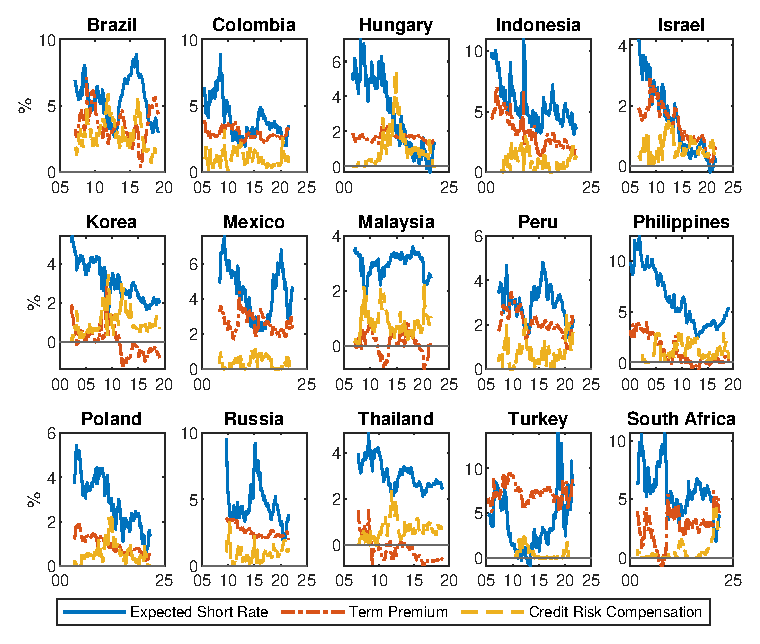
\includegraphics[trim={0cm 0cm 0cm 0cm},clip,height=0.8\textheight,width=\linewidth]{../Figures/ny_dcmp.eps} \\
					\end{center}
					\fignotes{This figure plots the components of the 10-year nominal yields of emerging markets. The yields are decomposed into an average expected future short-term interest rate (solid line), a term premium (dash-dotted line) and credit risk compensation (dashed line).}
				\end{minipage}
			\end{center}
		\end{figure}
	\end{landscape}
}

Finally, the components of the nominal yields of emerging markets are individually sensible. The model-implied 10-year average expected future short rate follows closely the (inferred) long-term forecast for the short rate. The model-implied term premium is positively correlated with a model-free term premium and with a common measure of inflation uncertainty as in \cite{Wright:2011}. The credit risk compensation is highly correlated with the LC credit spread of \cite{DuSchreger:2016JoF}. The online appendix \ref{sec:assessment} assesses each component individually as well as the robustness of the decomposition. 


\section{U.S. Monetary Policy Spillovers to Emerging Market Yields} \label{sec:analysis}
This section uses the three-part yield decomposition to analyze the transmission channels of U.S. monetary policy to emerging market yields. Surprises in U.S. monetary policy lead to a reassessment of policy rate expectations and a repricing of interest rate and credit risks in emerging markets. The evidence also shows that central banks in emerging markets exert relatively more control over the short end of their yield curves. 

\subsection{Transmission Channels} \label{sec:LPs} 
The following panel local projections assess the transmission of U.S. monetary policy to the yields of emerging markets 
\begin{equation} \label{eq:nPanelLP}
\eqpanelLP,
\end{equation}
\noindent in which \(\idxh\) indicates the horizon (in days) with \(\idxh = 0, 1, \ldots, 45\) and each \(\epsilon^{j}_{\idxt}\) represents one of the three types of monetary policy surprises described in section \ref{sec:USMPS}; even though the surprises are uncorrelated by construction, the estimation is more efficient when the three types of surprises are included simultaneously. The regressions include country fixed effects \(\alpha_{\idxh,\idxi}\), a lag of the exchange rate \(\fx_{\idxspnllag}\) to rule out explanations due to currency movements, and a lag of the dependent variable. As argued by \cite{HofmannShimShin:2020}, the large number of daily observations reduces the potential for Nickell bias that arises by including a lagged dependent variable in panel regressions with fixed effects and small time dimensions; indeed, the impulse responses are essentially the same when the lag of the dependent variable is excluded. The dependent variables are the 10- and 2-year nominal yields and each of their components. The confidence bands are constructed using Driscoll--Kraay standard errors, which allow for time and cross-sectional dependence. % Lags for DK in LPs: 9

The parameters of interest, \(\beta^{j}_{\idxh}\), measure the average response of the nominal yield and each of its components to monetary policy surprise \(j\) at horizon \(\idxh\). All responses are assessed relative to a one basis point reduction (an easing) in any of the surprises, since the Fed has been more aggressive in that direction over the sample period (see table \ref{tab:mpsstats}). 

The response of U.S. yields and their components to the three surprises serves as a benchmark to assess the responses of the yields of emerging markets. The components of U.S. yields come from the decomposition of \cite{KimWright:2005}, which uses survey forecasts of future short rates. Figures \ref{fig:LPUStarget} to \ref{fig:LPUSpathWh} in the online appendix show that the responses are consistent with the findings in the existing literature. Namely, target easing surprises reduce the yields, mainly driven by a decline in the average expected future short rates; while forward guidance and asset purchase easing surprises decrease yields, in part due to a reduction in the term premium. 

To better assess the cross-country heterogeneity, figures \ref{fig:LPLAEEtarget} to \ref{fig:LPEAMAlsap} in the online appendix report the responses to the three surprises of the 10-year yields grouped by regions. The regions are Latin America (Brazil, Colombia, Mexico, Peru), Emerging Europe (Hungary, Poland, Russia), Emerging Asia (Indonesia, Korea, Malaysia, Philippines, Thailand), and the Middle East and Africa (Israel, Turkey, South Africa). 

\subsubsection{Target Surprises}
Figure \ref{fig:LPEMtarget} shows that the response of emerging market yields to a target easing surprise builds over time. This delayed response is documented by \cite{BrooksKatzLustig:2019} for the U.S. and by \cite{ACDM:2019} for a sample mostly comprising advanced economies, which they attribute to a portfolio rebalancing channel and slow-moving capital; that is, some players (like pension funds and foreign investors) might respond gradually even though the U.S. Treasuries market is deep and liquid. As discussed later, the reaction of emerging market yields to forward guidance and asset purchase surprises is sluggish too. Slow-moving capital is thus also present in the bond markets of emerging economies. 

\afterpage{
	\begin{landscape}
		
		\begin{figure}[tbph]
			\caption{Response of the Yield Curve to a Target Surprise} \label{fig:LPEMtarget}
			\begin{center}
				\begin{minipage}{\linewidth}
					\begin{center}
						\begin{subfigure}[t]{\linewidth}
							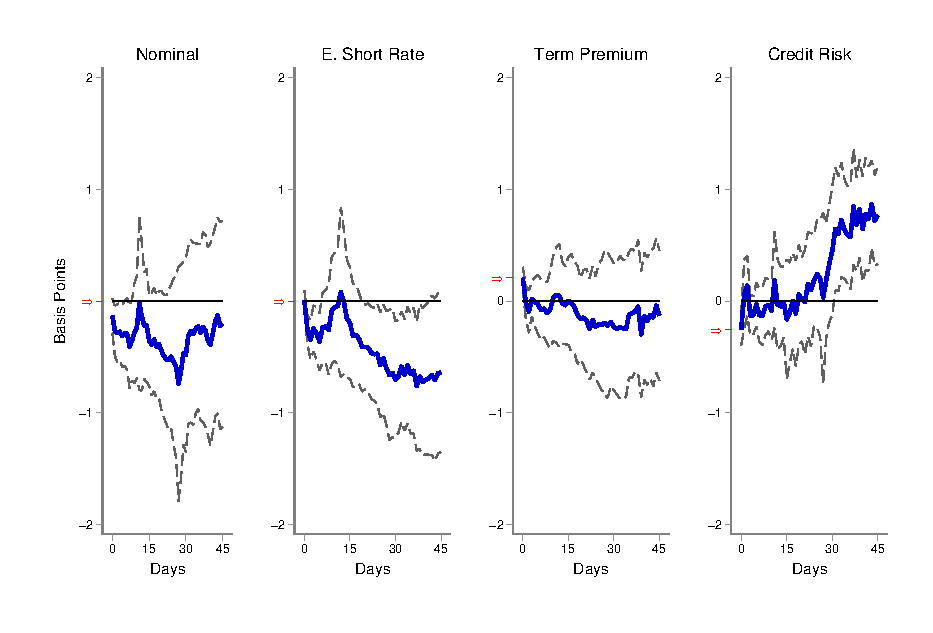
\includegraphics[trim={0cm 0cm 0cm 0cm},clip,height=0.35\textheight,width=\linewidth]{../Figures/TargetEMnomyptpphi120m.eps} \\
							\vspace{-0.35cm}
							\caption{10-Year Yield} \label{subfig:LPEM10Ytarget}
							\vspace{0.4cm}
						\end{subfigure}
						
						
						\begin{subfigure}[t]{\linewidth}
							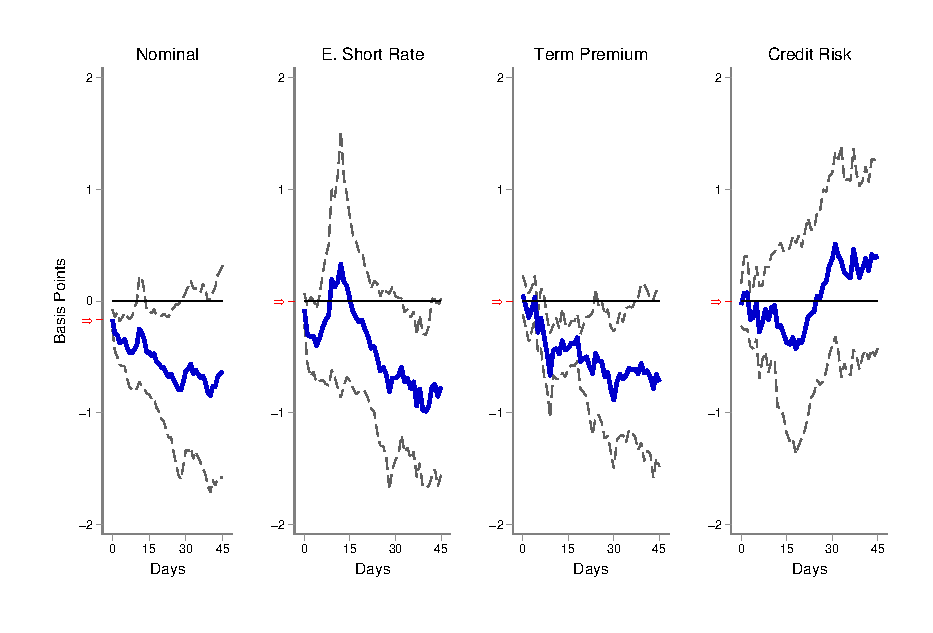
\includegraphics[trim={0cm 0cm 0cm 0cm},clip,height=0.35\textheight,width=\linewidth]{../Figures/TargetEMnomyptpphi24m.eps} \\
							\vspace{-0.35cm}
							\caption{2-Year Yield} \label{subfig:LPEM2Ytarget}
						\end{subfigure}
						\vspace{-0.45cm}
					\end{center}
					\fignotes{This figure shows the response of the 10- and 2-year emerging market nominal yields and their components to a target easing surprise of 1 basis point. Nominal yields are decomposed into an expected future short-term interest rate, a term premium and credit risk compensation, see section \ref{sec:Decomposition} for details. Target surprises are identified using intraday data around U.S. monetary policy announcements, see section \ref{sec:USMPS} for details. The 90\% confidence bands are based on Driscoll--Kraay standard errors.}
				\end{minipage}
			\end{center}
		\end{figure}
		
		\pagebreak[4]
		
		\begin{figure}[tbph]
			\caption{Response of the Yield Curve to a Forward Guidance Surprise: 2000-2008} \label{fig:LPEMpathPre}
			\begin{center}
				\begin{minipage}{\linewidth}
					\begin{center}
						\begin{subfigure}[t]{\linewidth}
							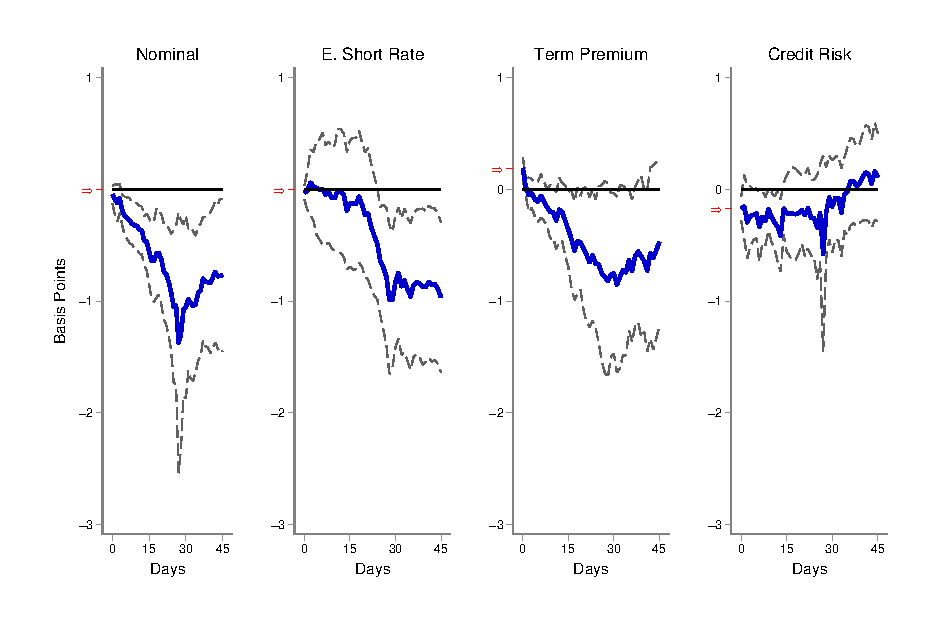
\includegraphics[trim={0cm 0cm 0cm 0cm},clip,height=0.35\textheight,width=\linewidth]{../Figures/PathEMnomyptpphi120mPre.eps} \\
							\vspace{-0.35cm}
							\caption{10-Year Yield} \label{subfig:LPEM10YpathPre}
						\end{subfigure}
						
						\vspace{0.2cm}
						
						\begin{subfigure}[t]{\linewidth}
							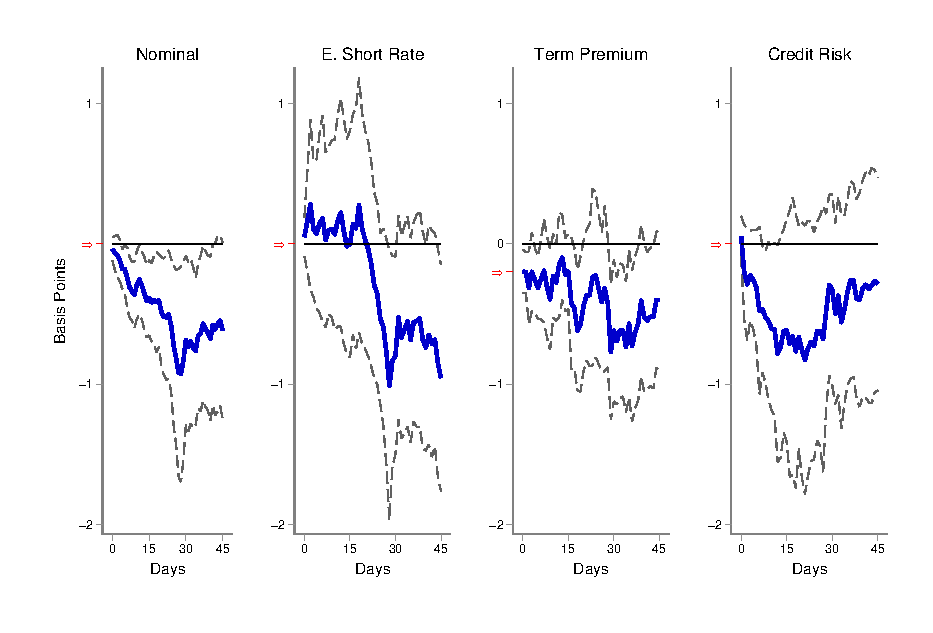
\includegraphics[trim={0cm 0cm 0cm 0cm},clip,height=0.35\textheight,width=\linewidth]{../Figures/PathEMnomyptpphi24mPre.eps} \\
							\vspace{-0.35cm}
							\caption{2-Year Yield} \label{subfig:LPEM2YpathPre}
						\end{subfigure}
						\vspace{-0.45cm}
					\end{center}
					\fignotes{This figure shows the response of the 10- and 2-year emerging market nominal yields and their components to a forward guidance easing surprise of 1 basis point. Nominal yields are decomposed into an expected future short-term interest rate, a term premium and credit risk compensation, see section \ref{sec:Decomposition} for details. Forward guidance surprises are identified using intraday data around U.S. monetary policy announcements, see section \ref{sec:USMPS} for details. The 90\% confidence bands are based on Driscoll--Kraay standard errors.}
				\end{minipage}
			\end{center}
		\end{figure}
		
		\pagebreak[4]
		
		\begin{figure}[tbph]
			\caption{Response of the Yield Curve to a Forward Guidance Surprise: 2008-2019} \label{fig:LPEMpathPost}
			\begin{center}
				\begin{minipage}{\linewidth}
					\begin{center}
						\begin{subfigure}[t]{\linewidth}
							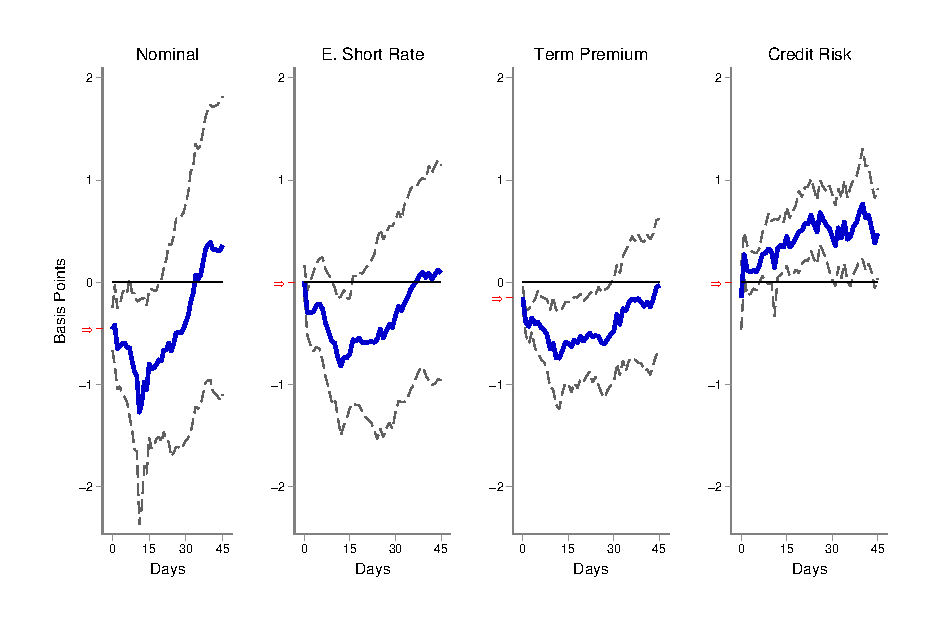
\includegraphics[trim={0cm 0cm 0cm 0cm},clip,height=0.35\textheight,width=\linewidth]{../Figures/PathEMnomyptpphi120mPost.eps} \\
							\vspace{-0.35cm}
							\caption{10-Year Yield} \label{subfig:LPEM10YpathPost}
						\end{subfigure}
						
						\vspace{0.2cm}
						
						\begin{subfigure}[t]{\linewidth}
							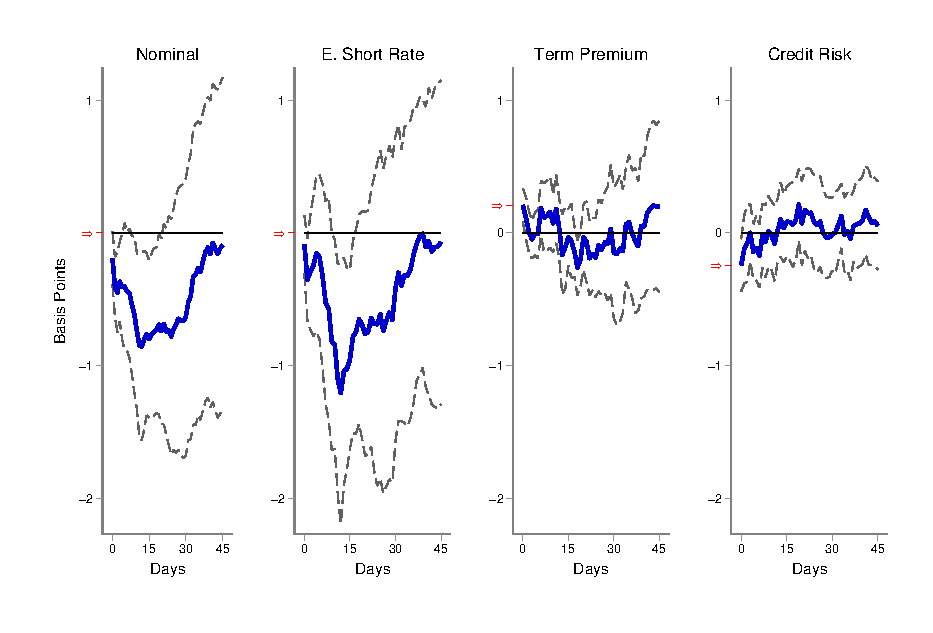
\includegraphics[trim={0cm 0cm 0cm 0cm},clip,height=0.35\textheight,width=\linewidth]{../Figures/PathEMnomyptpphi24mPost.eps} \\
							\vspace{-0.35cm}
							\caption{2-Year Yield} \label{subfig:LPEM2YpathPost}
						\end{subfigure}
						\vspace{-0.45cm}
					\end{center}
					\fignotes{This figure shows the response of the 10- and 2-year emerging market nominal yields and their components to a forward guidance easing surprise of 1 basis point. Nominal yields are decomposed into an expected future short-term interest rate, a term premium and credit risk compensation, see section \ref{sec:Decomposition} for details. Forward guidance surprises are identified using intraday data around U.S. monetary policy announcements, see section \ref{sec:USMPS} for details. The 90\% confidence bands are based on Driscoll--Kraay standard errors.}
				\end{minipage}
			\end{center}
		\end{figure}
		
		\pagebreak[4]
		
		\begin{figure}[tbph]
			\caption{Response of the Yield Curve to an Asset Purchase Surprise} \label{fig:LPEMlsap}
			\begin{center}
				\begin{minipage}{\linewidth}
					\begin{center}
						\begin{subfigure}[t]{\linewidth}
							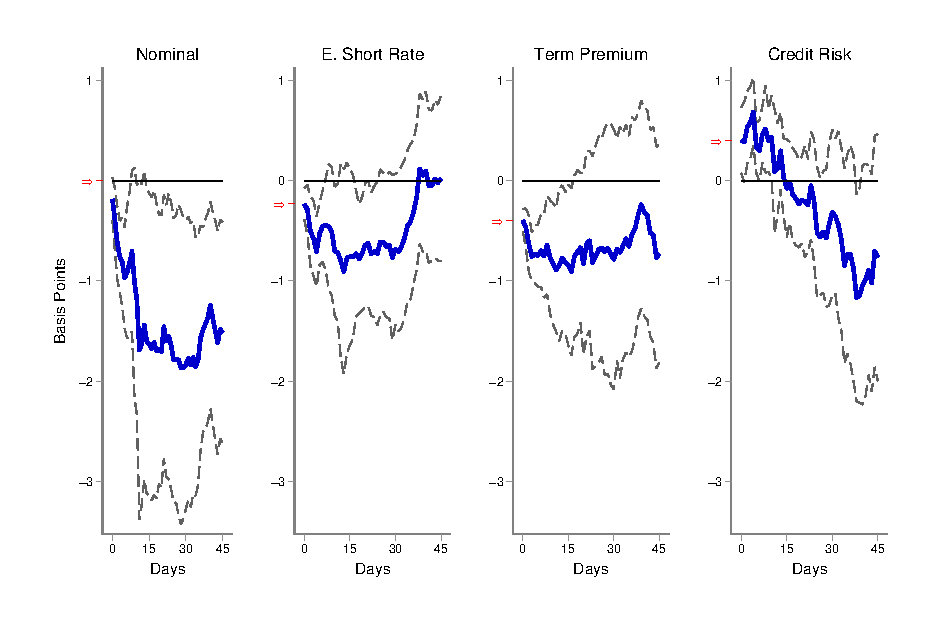
\includegraphics[trim={0cm 0cm 0cm 0cm},clip,height=0.35\textheight,width=\linewidth]{../Figures/LSAPEMnomyptpphi120m.eps} \\
							\vspace{-0.35cm}
							\caption{10-Year Yield} \label{subfig:LPEM10Ylsap}
						\end{subfigure}
						
						\vspace{0.2cm}
						
						\begin{subfigure}[t]{\linewidth}
							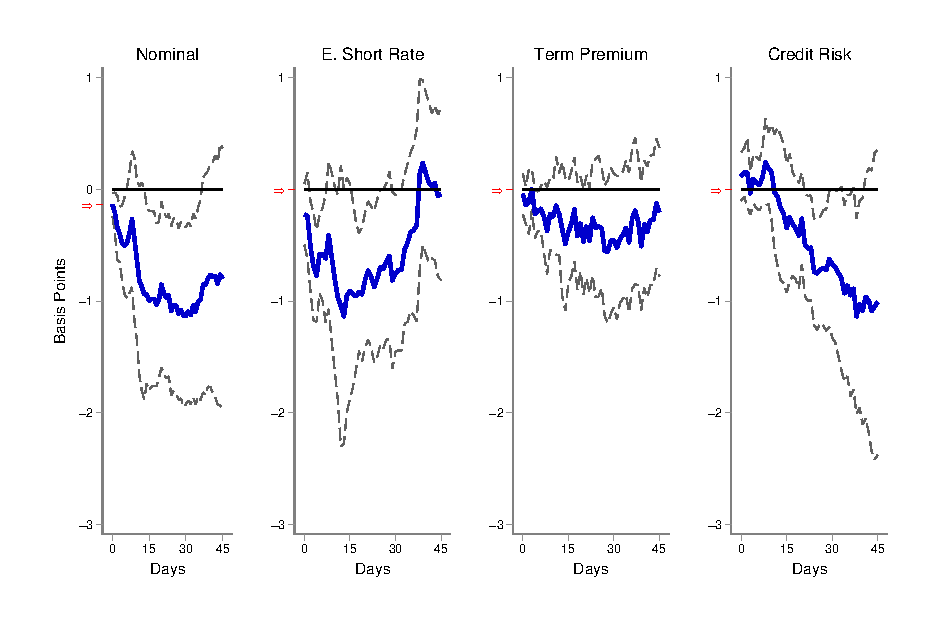
\includegraphics[trim={0cm 0cm 0cm 0cm},clip,height=0.35\textheight,width=\linewidth]{../Figures/LSAPEMnomyptpphi24m.eps} \\
							\vspace{-0.35cm}
							\caption{2-Year Yield} \label{subfig:LPEM2Ylsap}
						\end{subfigure}
						\vspace{-0.45cm}
					\end{center}
					\fignotes{This figure shows the response of the 10- and 2-year emerging market nominal yields and their components to an asset purchase easing surprise of 1 basis point. Nominal yields are decomposed into an expected future short-term interest rate, a term premium and credit risk compensation, see section \ref{sec:Decomposition} for details. Asset purchase surprises are identified using intraday data around U.S. monetary policy announcements, see section \ref{sec:USMPS} for details. The 90\% confidence bands are based on Driscoll--Kraay standard errors.}
				\end{minipage}
			\end{center}
		\end{figure}
		
	\end{landscape}
}

Figure \ref{fig:LPEMtarget} characterizes the response of emerging market yields to a target easing surprise. Investors expect central banks in emerging markets to follow the monetary stance of the Fed rather than counteract it, as can be seen in the eventual decline of the expected future short rate at both ends. The term premia at the short end also declines a few days after the surprise. Meanwhile, the credit risk compensation is an important factor to understand the transmission of U.S. monetary policy to emerging market yields. 

U.S. monetary policy alters the pricing of sovereign credit risk in emerging markets. While there is no effect on the credit risk compensation at the short end, it increases at the long end one month after the surprise (driven by the European and Asian countries, see figures \ref{fig:LPLAEEtarget} and \ref{fig:LPEAMAtarget}), reflecting either an increase in the price or the quantity of such risk. On the one hand, \cite{JeanneretSouissi:2016} show that global factors affect investors’ compensation for holding sovereign credit risk, not the risk itself; on the other, loose financial conditions in the U.S. trigger a `reach-for-yield' behavior among investors \citep{HausmanWongswan:2011} that incentivizes more borrowing in emerging markets by sovereigns in local currency \citep{BigioNunoPassadore:2018} and corporates in foreign currency \citep{Turner:2014}, increasing the sovereign default risk in emerging markets \citep{DuSchreger:2022RFS}. In any case, U.S. monetary policy could be seen as having fiscal implications in emerging markets, a previously overlooked channel. 

\subsubsection{Forward Guidance Surprises}
Since U.S. monetary policy spillovers to long-term yields increased after the global financial crisis \citep{Albaglietal:2019}, figures \ref{fig:LPEMpathPre} and \ref{fig:LPEMpathPost} display the responses to a forward guidance easing surprise before and after October 2008, respectively. Figure \ref{fig:LPEMpathWh} in the online appendix reports the results for the whole period. All the responses are sluggish. 

The transmission of forward guidance easing surprises changed. Before the global financial crisis, a forward guidance easing surprise led to a downward parallel shift in the yield curves of emerging markets; the effect lasted longer than on U.S. yields (cf. figure \ref{fig:LPUSpathPre}), and was generally driven by declines in both the expected future short rate and the term premium. After the global financial crisis, the reduction in the expected future short rate mainly happens at the short end, whereas the drop in the term premium occurs only at the long end, as is generally expected with unconventional easing policies. Moreover, the nominal yield curve in emerging markets steepens relative to the U.S. yield curve in the month following the surprise (cf. figure \ref{fig:LPUSpathPost}), so the nominal-synthetic spread in emerging markets widens at the long end, primarily in Asian countries (see figure \ref{fig:LPEAMApath}). Loose future financial conditions therefore increase the price or the quantity of default risk similar to target easing surprises. 

The characterization of the response of the term premia to forward guidance surprises is where accounting for credit risk pays off. By signaling a loose future path for the federal funds rate, the Fed attempts to reduce long-term U.S. yields mainly by reducing the term premium (see figure \ref{fig:LPUSpathPost}). Figure \ref{fig:LPEMpathPost} shows that the response of the term premia is similar in emerging markets than in the U.S., since forward guidance easing surprises also reduce the term premia in emerging market yields at the long end, in line with \cite{Turner:2014}. If, instead, credit risk were to be ignored, one would incorrectly conclude that forward guidance does not affect the term premia in emerging markets. The reason is that the `clean' term premium and the credit risk compensation components respond in opposite directions with magnitudes that almost offset each other, so there is no net effect in the term premium contaminated with credit risk.

\subsubsection{Asset Purchase Surprises}
Figure \ref{fig:LPEMlsap} displays the response of emerging market yields to an asset purchase easing surprise. Asset purchase surprises not only give rise to sluggish responses in the yields, as target and forward guidance surprises do, but their effects last longer in emerging market yields than in U.S. yields (cf. figure \ref{fig:LPUSlsap}). This result suggests that portfolio rebalancing due to asset purchases is slower in emerging markets.

An asset purchase easing surprise flattens the yield curve in emerging markets, similar to the effect on the U.S. yield curve (see figure \ref{fig:LPUSlsap}). In both cases, the effect at the long end is larger than at the short end. The on-impact response of U.S. yields is larger, whereas the response of the nominal yields of emerging markets lasts longer. These two effects in turn explain the response of the credit risk compensation at the long end, which initially increases followed by a sluggish and considerable decline. The counterintuitive initial increase is more a reflection of the response in the U.S. Treasuries market than on the bond markets in emerging economies. Indeed, an asset purchase easing surprise triggers a strong investor reaction in the U.S. Treasuries market, leading to a  more than one-to-one on-impact decline in the long-term U.S. yield (see figure \ref{subfig:LPUS10Ylsap}). 

The response of the term premium to an asset purchase easing surprise is similar in emerging markets than in the U.S. Specifically, the term premium declines at the long end, as with a forward guidance easing surprise after the global financial crisis. In addition, the decline occurs across emerging market regions (see figures \ref{fig:LPLAEElsap} and \ref{fig:LPEAMAlsap}). 

Overall, U.S. monetary policy is an important driver of emerging market yields as it influences all of their components. Moreover, unconventional easing policies in the U.S. spread abroad, and their spillovers are more persistent than conventional policies. 

\subsection{The Yield Curve Channel} \label{sec:Drivers}
The U.S. monetary policy influence on emerging market yields can also be seen through the link between the yield components, henceforth referred to as the yield curve channel. The literature describes different mechanisms. \cite{Obstfeld:2015} argues that central banks exert more control over the short end of their yield curves because long-term yields are more influenced by global forces than short-term ones. Meanwhile, changes in the U.S. term premium can spill over into emerging market yields via the term premium \citep{Turner:2014}, and the expected future short rate due to risk spillovers \citep{Kalemli-Ozcan:2019}. Thus, emerging markets remain vulnerable to global risks even when they borrow in LC. 

To assess the role of the components of U.S. yields (the average expected future short rate and the term premium) on the components of emerging market yields at different maturities, I run the following panel regressions using monthly data 
\begin{equation} \label{eq:nPanelDCMP}
\eqpanelTPreg ,
\end{equation}
\noindent in which \(\alpha_{\idxi}\) are country fixed effects, \(z^{1}_{\idxspnl}\) is a vector containing the components of the U.S. yield curve, \(z^{2}_{\idxspnl}\) is a vector of global and domestic variables as potential drivers of emerging market yields, and \(u_{\idxspnl}\) is the error term. The dependent variable \(\yld_{\idxspnl}\) is either the nominal yield or any of its three components for the 10- and 2-year maturities. As before, I use Driscoll--Kraay standard errors to test for significance. 

The main explanatory variables are the components of U.S. yields (at corresponding maturities) form the decomposition of \cite{KimWright:2005}. The controls for the local macroeconomic conditions are the policy rate reported by the Bank for International Settlements, as well as the domestic inflation and unemployment rates. The (standardized) exchange rate in each country rules out explanations of changes in yields due to currency movements. The Cboe Volatility Index (VIX) is included as an important driver of the global financial cycle \citep{Rey:2013}. Alternative, and arguably exogenous, measures of global uncertainty are the global and U.S. versions of the news-based economic policy uncertainty (EPU) index of \cite{BakerBloomDavis:2016}. The VIX and EPU indices are used in logs. Finally, the global economic activity index of \cite{Hamilton:2021} captures real variables. 

Tables \ref{tab:ycdcmp10y} and \ref{tab:ycdcmp2y} report the results. Notice that the term premium and the credit risk compensation are not only associated with local (inflation, unemployment rate) and global (VIX, EPU U.S.) factors but with the components of U.S. yields. 

The direct and cross relationships between the components of U.S. and emerging market yields are in line with the yield curve channel. On the one hand, the response of the average expected future short rates of emerging markets to the domestic policy rate decreases with maturity and is positively associated with its U.S. counterpart only at the long end. The online appendix \ref{sec:comovement} further shows that the long-term yields of emerging markets comove more than short-term ones. Thus, in line with \cite{Obstfeld:2015}, monetary autonomy is stronger at the short end than at the long end of the curve. 

\begin{normalsize}
	\begin{table}
		\begin{center}
			\caption{Drivers of the Emerging Market 10-Year Nominal Yield and Its Components} \label{tab:ycdcmp10y}
			\begin{threeparttable}
				\begin{tabularx}{0.95\linewidth}{l*{6}C}
					\toprule
					&\multicolumn{1}{c}{Nominal}&\multicolumn{1}{c}{E. Short Rate}&\multicolumn{1}{c}{Term Premium}&\multicolumn{1}{c}{Credit Risk}\\\cmidrule(lr){2-2}\cmidrule(lr){3-3}\cmidrule(lr){4-4}\cmidrule(lr){5-5}
					U.S. Term Premium   &        0.76\sym{*}  &        0.26         &        0.74\sym{***}&       -0.19         \\
					&      (0.36)         &      (0.22)         &      (0.18)         &      (0.12)         \\
					U.S. E. Short Rate  &       -0.54\sym{*}  &       -0.11         &       -0.38\sym{*}  &       -0.13         \\
					&      (0.24)         &      (0.18)         &      (0.15)         &      (0.08)         \\
					Local Policy Rate   &        0.17\sym{**} &        0.32\sym{***}&       -0.02         &       -0.07\sym{***}\\
					&      (0.06)         &      (0.04)         &      (0.03)         &      (0.02)         \\
					Inflation           &        9.55\sym{**} &        7.87\sym{**} &       -4.52         &        4.99\sym{***}\\
					&      (3.50)         &      (2.66)         &      (2.56)         &      (1.46)         \\
					Unemployment        &       30.91\sym{***}&        2.41         &       21.42\sym{***}&        3.11         \\
					&      (5.18)         &      (4.55)         &      (3.39)         &      (2.42)         \\
					LC per USD (Std.)   &       52.86\sym{***}&       65.12\sym{***}&       -4.03         &        0.28         \\
					&     (14.23)         &      (8.06)         &      (7.77)         &      (8.28)         \\
					Log(VIX)            &      -32.59         &        8.22         &      -43.14\sym{**} &        2.12         \\
					&     (25.96)         &     (15.79)         &     (14.65)         &      (8.14)         \\
					Log(EPU U.S.)       &       -0.61         &        0.43         &       -1.03         &        1.06         \\
					&      (9.79)         &      (5.47)         &      (5.04)         &      (3.63)         \\
					Log(EPU Global)     &      -18.74         &      -34.85         &      -15.31         &       26.54         \\
					&     (40.29)         &     (30.53)         &     (30.53)         &     (15.70)         \\
					Global Ind. Prod.   &        7.22\sym{*}  &       10.55\sym{***}&       -3.14         &        2.15         \\
					&      (3.33)         &      (2.12)         &      (1.66)         &      (1.85)         \\\midrule
					Fixed Effects       &         Yes         &         Yes         &         Yes         &         Yes         \\
					Lags                &           3         &           3         &           3         &           3         \\
					No. Countries       &           9         &           9         &           9         &           9         \\
					Observations        &         468         &         468         &         468         &         468         \\
					\(R^{2}\)           &        0.51         &        0.49         &        0.52         &        0.12         \\
					\bottomrule
					\addlinespace[.75ex]
				\end{tabularx}
				\tabnote{This table reports the estimated slope coefficients of panel data regressions of the 10-year nominal yield and its components (expected short rate, term premium and credit risk compensation) on selected explanatory variables. The sample includes monthly data for 15 emerging markets starting in 2000:1 and ending in 2021:7. The dependent variables are expressed in basis points. The explanatory variables are the U.S. term premium and the U.S. expected short rate according to \cite{KimWright:2005} with the same maturity as the dependent variables, the policy rate, domestic inflation and unemployment rates, the standardized exchange rate (LC per USD), the log of the VIX, the log of the U.S. and global economic policy uncertainty indexes based on \cite{BakerBloomDavis:2016}, the global economic activity index of \cite{Hamilton:2021}. Driscoll--Kraay standard errors in parenthesis. The lag length up to which the residuals may be autocorrelated is indicated. *, **, *** asterisks respectively indicate significance at the 10\%, 5\% and 1\% level.}
			\end{threeparttable}
		\end{center}
	\end{table}
\end{normalsize}

\begin{normalsize}
	\begin{table}
		\begin{center}
			\caption{Drivers of the Emerging Market 2-Year Nominal Yield and Its Components} \label{tab:ycdcmp2y}
			\begin{threeparttable}
				\begin{tabularx}{0.95\linewidth}{l*{6}C}
					\toprule
					&\multicolumn{1}{c}{Nominal}&\multicolumn{1}{c}{E. Short Rate}&\multicolumn{1}{c}{Term Premium}&\multicolumn{1}{c}{Credit Risk}\\\cmidrule(lr){2-2}\cmidrule(lr){3-3}\cmidrule(lr){4-4}\cmidrule(lr){5-5}
					U.S. Term Premium   &        1.73\sym{***}&        1.55\sym{***}&        0.23         &       -0.19         \\
					&      (0.19)         &      (0.22)         &      (0.13)         &      (0.18)         \\
					U.S. E. Short Rate  &       -0.02         &        0.05         &        0.06\sym{***}&       -0.14\sym{***}\\
					&      (0.03)         &      (0.04)         &      (0.02)         &      (0.03)         \\
					Local Policy Rate   &        0.64\sym{***}&        0.67\sym{***}&       -0.00         &        0.01         \\
					&      (0.02)         &      (0.03)         &      (0.01)         &      (0.02)         \\
					Inflation           &        7.26\sym{**} &        4.15         &        4.09\sym{*}  &        1.57         \\
					&      (2.24)         &      (3.07)         &      (1.66)         &      (1.81)         \\
					Unemployment        &        6.11\sym{**} &        0.71         &        0.75         &        5.25\sym{**} \\
					&      (2.20)         &      (2.70)         &      (1.26)         &      (1.63)         \\
					LC per USD (Std.)   &       24.36\sym{***}&       27.19\sym{***}&       21.60\sym{***}&      -14.43\sym{**} \\
					&      (5.06)         &      (5.37)         &      (3.19)         &      (4.64)         \\
					Log(VIX)            &       45.06\sym{***}&       -3.22         &      -13.84\sym{*}  &       62.28\sym{***}\\
					&      (7.33)         &     (14.30)         &      (5.85)         &     (11.57)         \\
					Log(EPU U.S.)       &        6.31         &       -4.79         &       -2.43         &       10.92\sym{**} \\
					&      (3.76)         &      (5.21)         &      (2.24)         &      (3.85)         \\
					Log(EPU Global)     &      -53.73\sym{***}&      -34.24\sym{**} &       -6.50         &       -9.61         \\
					&     (12.73)         &     (12.25)         &      (6.99)         &      (9.18)         \\
					Global Ind. Prod.   &        2.34\sym{***}&       -1.94\sym{*}  &        0.17         &        3.40\sym{***}\\
					&      (0.59)         &      (0.97)         &      (0.47)         &      (0.77)         \\\midrule
					Fixed Effects       &         Yes         &         Yes         &         Yes         &         Yes         \\
					Lags                &           4         &           4         &           4         &           4         \\
					No. Countries       &          15         &          15         &          15         &          15         \\
					Observations        &        2493         &        2493         &        2493         &        2493         \\
					\(R^{2}\)           &        0.82         &        0.78         &        0.18         &        0.30         \\
					\bottomrule
					\addlinespace[.75ex]
				\end{tabularx}
				\tabnote{This table reports the estimated slope coefficients of panel data regressions of the 2-year nominal yield and its components (expected short rate, term premium and credit risk compensation) on selected explanatory variables. The sample includes monthly data for 15 emerging markets starting in 2000:1 and ending in 2021:7. The dependent variables are expressed in basis points. The explanatory variables are the U.S. term premium and the U.S. expected short rate according to \cite{KimWright:2005} with the same maturity as the dependent variables, the policy rate, domestic inflation and unemployment rates, the standardized exchange rate (LC per USD), the log of the VIX, the log of the U.S. and global economic policy uncertainty indexes based on \cite{BakerBloomDavis:2016}, the global economic activity index of \cite{Hamilton:2021}. Driscoll--Kraay standard errors in parenthesis. The lag length up to which the residuals may be autocorrelated is indicated. *, **, *** asterisks respectively indicate significance at the 10\%, 5\% and 1\% level.}
			\end{threeparttable}
		\end{center}
	\end{table}
\end{normalsize}

On the other hand, the U.S. term premium is an important driver of emerging market yields. First, their term premia are positively associated with the U.S. term premium and the VIX only at the long end, so that the global financial cycle (represented here by those two variables) is more relevant for the long end than for the short end of the curve \citep{Obstfeld:2015}. Second, the U.S. term premium not only influences the yields in emerging markets through its effect on their term premia, as suggested by \cite{Turner:2014}, but through the other components too. In particular, its influence on the average expected future short rates of emerging markets supports the risk spillovers mechanism highlighted by \cite{Kalemli-Ozcan:2019}, which can be directly tested thanks to the yield decompositions. Moreover, those risk spillovers are stronger at the short end and operate through the U.S. term premium rather than the VIX. Importantly, these results would differ if the default risk were to be ignored since the term premium and the credit risk compensation would be mixed together. 


\section{Concluding Remarks} \label{sec:conclusions}
This paper decomposes the sovereign yields of 15 emerging markets into three parts (an average expected future short rate, a term premium and compensation for credit risk) to adequately quantify the transmission channels of U.S. monetary policy. 

Surprises in U.S. monetary policy lead to a reassessment of policy rate expectations and a repricing of interest rate and credit risks in emerging markets. Specifically, investors expect monetary authorities in emerging markets to follow the monetary stance of the Fed rather than counteract it, the response of emerging market term premia to unconventional policies is similar to that of the U.S. term premium, and U.S. monetary policy also alters the pricing of sovereign credit risk in emerging markets. 

The analysis in this paper can be extended in several directions. The proposed three-part decomposition of emerging market yields has many potential applications, including the analysis of the transmission of monetary policy domestically or the monetary policy spillovers of other central banks. The effect on credit risk may also inform theoretical models for pricing sovereign defaultable bonds. 


\section*{Acknowledgments}
\begin{spacing}{1.25} 
I thank Jonathan Wright for his invaluable advice, to Greg Duffee and Olivier Jeanne for insightful suggestions, to the editors and two anonymous referees for their valuable feedback. I also thank Tobias Adrian, Derin Aksit, Laurence Ball, Bob Barbera, Christopher Carroll, Lalit Contractor, Alejandro Díaz de León, Jon Faust, Jorge Luis García Ramírez, Fabrizio López Gallo Dey, Daniel Millimet, Alessandro Rebucci, Tatjana Schulze, and seminar participants at Johns Hopkins University, Loyola University, Carey Business School, the Bank of Spain, the Bank of Mexico, the CNBV, the 2021 Finance Research Letters Virtual Conference and the 2021 EEA-ESEM Virtual Congress for their helpful comments and suggestions. All remaining errors are mine. 
\end{spacing}

%---------------------------------------------------------------
% References
%---------------------------------------------------------------
\newpage
\bibliographystyle{abbrvnat}
	\bibliography{../References/library}

\end{document}